% Options for packages loaded elsewhere
\PassOptionsToPackage{unicode}{hyperref}
\PassOptionsToPackage{hyphens}{url}
\PassOptionsToPackage{dvipsnames,svgnames,x11names}{xcolor}
%
\documentclass[
  abstract]{article}

\usepackage{amsmath,amssymb}
\usepackage{setspace}
\usepackage{iftex}
\ifPDFTeX
  \usepackage[T1]{fontenc}
  \usepackage[utf8]{inputenc}
  \usepackage{textcomp} % provide euro and other symbols
\else % if luatex or xetex
  \usepackage{unicode-math}
  \defaultfontfeatures{Scale=MatchLowercase}
  \defaultfontfeatures[\rmfamily]{Ligatures=TeX,Scale=1}
\fi
\usepackage{lmodern}
\ifPDFTeX\else  
    % xetex/luatex font selection
\fi
% Use upquote if available, for straight quotes in verbatim environments
\IfFileExists{upquote.sty}{\usepackage{upquote}}{}
\IfFileExists{microtype.sty}{% use microtype if available
  \usepackage[]{microtype}
  \UseMicrotypeSet[protrusion]{basicmath} % disable protrusion for tt fonts
}{}
\makeatletter
\@ifundefined{KOMAClassName}{% if non-KOMA class
  \IfFileExists{parskip.sty}{%
    \usepackage{parskip}
  }{% else
    \setlength{\parindent}{0pt}
    \setlength{\parskip}{6pt plus 2pt minus 1pt}}
}{% if KOMA class
  \KOMAoptions{parskip=half}}
\makeatother
\usepackage{xcolor}
\usepackage[top=30mm,left=30mm,bottom=30mm,right=30mm,heightrounded]{geometry}
\setlength{\emergencystretch}{3em} % prevent overfull lines
\setcounter{secnumdepth}{-\maxdimen} % remove section numbering
% Make \paragraph and \subparagraph free-standing
\ifx\paragraph\undefined\else
  \let\oldparagraph\paragraph
  \renewcommand{\paragraph}[1]{\oldparagraph{#1}\mbox{}}
\fi
\ifx\subparagraph\undefined\else
  \let\oldsubparagraph\subparagraph
  \renewcommand{\subparagraph}[1]{\oldsubparagraph{#1}\mbox{}}
\fi


\providecommand{\tightlist}{%
  \setlength{\itemsep}{0pt}\setlength{\parskip}{0pt}}\usepackage{longtable,booktabs,array}
\usepackage{calc} % for calculating minipage widths
% Correct order of tables after \paragraph or \subparagraph
\usepackage{etoolbox}
\makeatletter
\patchcmd\longtable{\par}{\if@noskipsec\mbox{}\fi\par}{}{}
\makeatother
% Allow footnotes in longtable head/foot
\IfFileExists{footnotehyper.sty}{\usepackage{footnotehyper}}{\usepackage{footnote}}
\makesavenoteenv{longtable}
\usepackage{graphicx}
\makeatletter
\def\maxwidth{\ifdim\Gin@nat@width>\linewidth\linewidth\else\Gin@nat@width\fi}
\def\maxheight{\ifdim\Gin@nat@height>\textheight\textheight\else\Gin@nat@height\fi}
\makeatother
% Scale images if necessary, so that they will not overflow the page
% margins by default, and it is still possible to overwrite the defaults
% using explicit options in \includegraphics[width, height, ...]{}
\setkeys{Gin}{width=\maxwidth,height=\maxheight,keepaspectratio}
% Set default figure placement to htbp
\makeatletter
\def\fps@figure{htbp}
\makeatother
\newlength{\cslhangindent}
\setlength{\cslhangindent}{1.5em}
\newlength{\csllabelwidth}
\setlength{\csllabelwidth}{3em}
\newlength{\cslentryspacingunit} % times entry-spacing
\setlength{\cslentryspacingunit}{\parskip}
\newenvironment{CSLReferences}[2] % #1 hanging-ident, #2 entry spacing
 {% don't indent paragraphs
  \setlength{\parindent}{0pt}
  % turn on hanging indent if param 1 is 1
  \ifodd #1
  \let\oldpar\par
  \def\par{\hangindent=\cslhangindent\oldpar}
  \fi
  % set entry spacing
  \setlength{\parskip}{#2\cslentryspacingunit}
 }%
 {}
\usepackage{calc}
\newcommand{\CSLBlock}[1]{#1\hfill\break}
\newcommand{\CSLLeftMargin}[1]{\parbox[t]{\csllabelwidth}{#1}}
\newcommand{\CSLRightInline}[1]{\parbox[t]{\linewidth - \csllabelwidth}{#1}\break}
\newcommand{\CSLIndent}[1]{\hspace{\cslhangindent}#1}

\usepackage{lscape} \newcommand{\blandscape}{\begin{landscape}} \newcommand{\elandscape}{\end{landscape}} \renewcommand{\abstractname}{Abstract} \usepackage{booktabs} \usepackage{siunitx} \newcolumntype{d}{S[ input-open-uncertainty=, input-close-uncertainty=, parse-numbers = false, table-align-text-pre=false, table-align-text-post=false ]}
\makeatletter
\makeatother
\makeatletter
\makeatother
\makeatletter
\@ifpackageloaded{caption}{}{\usepackage{caption}}
\AtBeginDocument{%
\ifdefined\contentsname
  \renewcommand*\contentsname{Table of contents}
\else
  \newcommand\contentsname{Table of contents}
\fi
\ifdefined\listfigurename
  \renewcommand*\listfigurename{List of Figures}
\else
  \newcommand\listfigurename{List of Figures}
\fi
\ifdefined\listtablename
  \renewcommand*\listtablename{List of Tables}
\else
  \newcommand\listtablename{List of Tables}
\fi
\ifdefined\figurename
  \renewcommand*\figurename{Figure}
\else
  \newcommand\figurename{Figure}
\fi
\ifdefined\tablename
  \renewcommand*\tablename{Table}
\else
  \newcommand\tablename{Table}
\fi
}
\@ifpackageloaded{float}{}{\usepackage{float}}
\floatstyle{ruled}
\@ifundefined{c@chapter}{\newfloat{codelisting}{h}{lop}}{\newfloat{codelisting}{h}{lop}[chapter]}
\floatname{codelisting}{Listing}
\newcommand*\listoflistings{\listof{codelisting}{List of Listings}}
\makeatother
\makeatletter
\@ifpackageloaded{caption}{}{\usepackage{caption}}
\@ifpackageloaded{subcaption}{}{\usepackage{subcaption}}
\makeatother
\makeatletter
\@ifpackageloaded{tcolorbox}{}{\usepackage[skins,breakable]{tcolorbox}}
\makeatother
\makeatletter
\@ifundefined{shadecolor}{\definecolor{shadecolor}{rgb}{.97, .97, .97}}
\makeatother
\makeatletter
\makeatother
\makeatletter
\makeatother
\ifLuaTeX
  \usepackage{selnolig}  % disable illegal ligatures
\fi
\IfFileExists{bookmark.sty}{\usepackage{bookmark}}{\usepackage{hyperref}}
\IfFileExists{xurl.sty}{\usepackage{xurl}}{} % add URL line breaks if available
\urlstyle{same} % disable monospaced font for URLs
\hypersetup{
  pdftitle={CONSTITUTIONAL CHANGES UNDER POPULIST GOVERNMENTS},
  pdfauthor={Jasmin Sarah König; Tilko Swalve},
  colorlinks=true,
  linkcolor={blue},
  filecolor={Maroon},
  citecolor={Blue},
  urlcolor={Blue},
  pdfcreator={LaTeX via pandoc}}

\title{CONSTITUTIONAL CHANGES UNDER POPULIST GOVERNMENTS}
\usepackage{etoolbox}
\makeatletter
\providecommand{\subtitle}[1]{% add subtitle to \maketitle
  \apptocmd{\@title}{\par {\large #1 \par}}{}{}
}
\makeatother
\subtitle{An Empirical Analysis}
\author{Jasmin Sarah König\footnote{University of Hamburg. Jasmin wurde
  durch die Deutsche Forschungsgemeinschaft (DFG) -- GRK 2503 gefördert.
  Address for Correspondence jasmin.sarah.koenig@uni-hamburg.de} \and Tilko
Swalve\footnote{Leibniz University Hannover}}
\date{}

\begin{document}
\maketitle
\begin{abstract}
Despite significant judicial reforms under populist governments,
research on populism and constitutionalism is still under-developed.
Some scholars argue that populists aim to tie constitutional content to
will of the people. Others view the relationship as a purely
instrumental one and argue that populists aim to consolidate their power
through constitutional changes. We argue that, if populists want the
constitution to mirror the public's interests, we should observe more
constitutional changes once they are in power. Another question that
arises is what effect changes under populist governments have on
democratic quality. We argue that the heterogenous nature of populist
parties should be mirrored in different effects on democratic quality
depending on the government's ideological leaning. Using V-Dem, V-Party,
and CCP data, we estimate whether populists in power use constitutional
changes more frequently than other governments and what effects these
changes have on different aspects of democratic quality. We do not find
evidence that populists change the constitution more frequently than
other parties. However, we do find evidence that the effect of
constitutional changes under populist government differ depending on
their ideological leaning. While constitutional changes under left-wing
populist governments increase the quality of liberal democracy,
polyarchy, and egalitarianism, those under right-wing populists only
have a significant negative effect on egalitarianism.
\end{abstract}
\ifdefined\Shaded\renewenvironment{Shaded}{\begin{tcolorbox}[enhanced, sharp corners, frame hidden, interior hidden, boxrule=0pt, breakable, borderline west={3pt}{0pt}{shadecolor}]}{\end{tcolorbox}}\fi

\setstretch{1.5}
\newpage{}

\hypertarget{introduction}{%
\subsection{1. Introduction}\label{introduction}}

The relationship between populism and constitutionalism has been in the
centre of few but contentious debates. While some contend that populists
seek to empower the people through constitutional reform (Blokker,
2019a; Tushnet \& Bugaric, 2020; Tushnet \& Bugarič, 2021), others posit
that populists merely instrumentalize constitutional mechanisms to
consolidate their power (Mudde, 2021; Müller, 2017a; Rovira Kaltwasser,
2013). However, unlike the discourse surrounding populism and democracy,
this debate often lacks concrete empirical evidence to substantiate its
various claims. Our study aims to address this void by examining how
populist administrations enact and leverage constitutional change in
practice across 57 European and Latin American states.

In modern democracies, values and principles, such as the separation of
powers or civil rights, are often implemented in a constitution
(Habermas \& Rehg, 2001; Whittington, 2010). The codification of such
principles is supposed to constrain public authority and protect
citizens from state power (Stone Sweet, 2002). However, it also
constrains popular sovereignty by constraining the power of the
majority, for example, through checks and balances or minority rights.

The populist ideology, on the other hand, revolves around popular
sovereignty (Abts \& Rummens, 2007). Populists vow to give the power
back to the people. In populism, the outcome of politics not a
restriction of the latter (Blokker, 2019a; Mudde \& Rovira Kaltwasser,
2012a). Generally, one can distinguish two ways to think about the
relationship between populism and constitutionalism. Some scholars argue
that populism aims to democratize constitutions by increasing
participation and adapting the contents of the constitution to the
preferences of the majority (Blokker, 2019a; Tushnet \& Bugarič, 2021).
We call this the ideological approach. Others argue that populism has an
instrumental approach to constitutionalism. They contend that populists
adapt the constitution in ways it consolidates their power (Mudde, 2021;
Müller, 2017a; Rovira Kaltwasser, 2013).

We argue that, if populists are acting ideologically, we should observe
an increase in constitutional changes under populist governments. But,
if populists merely try to consolidate their power through
constitutional changes, the constitution does not need to be changed
more frequently. Few significant changes are sufficient to reach such a
goal.

Frequently, the decrease of democratic quality through constitutional
changes is linked with populists in power (Scheppele, 2019; see for
example Arato, 2019; Lacey, 2019). Thus, independent of the frequency of
constitutional changes, the question arises whether constitutional
changes have a different effect on democratic quality when populists are
in power compared to other governments. The heterogeneity of populist
parties makes it challenging to pin down their effects on democratic
quality (Huber \& Schimpf, 2017; Mény \& Surel, 2002; Mudde \& Rovira
Kaltwasser, 2012a, 2013). We argue that the ambiguity of populism is
likely to be mirrored in the effects of their constitutional amendments
on democratic quality. Depending on the democratic dimension under
consideration, the effect of populist constitutional reform is likely to
differ. Constitutional changes under left-wing populist governments are
likely to differ from those under right-wing populist governments.

We test both arguments with a dataset combined from Ruth--Lovell \&
Grahn (2023), the V-Dem (Coppedge et al., 2021) and V-Party (Lindberg et
al., 2022) as well as the Comparative Constitutions Project(Elkins et
al., 2021). We run fixed-effects panel models which do not show any
evidence in favor of the ideological approach to populism and
constitutionalism. Our results show that populists do not implement
constitutional changes more frequently than other governments,
independent of their ideology and government size. We show that the
effect of constitutional changes under populist governments differs
depending on whether they are left-, or right-leaning and the democratic
dimension under consideration. While constitutional changes under
left-wing populists have a significantly positive effect on liberal
democracy, polyarchy, and egalitarianism, those under right-wing
populists have a significantly negative effect on egalitarianism.

\hypertarget{populism-constitutionalism}{%
\subsection{2. POPULISM \&
CONSTITUTIONALISM}\label{populism-constitutionalism}}

The most commonly used definition of populism in Political Science
describes it as a thin ideology (Mudde, 2004). Populism usually emerges
tied to a ``denser'' host ideology, for example fascism or socialism,
and yet populism its own ideological core. The populist ideology is
based on the majority principle, in which only the ``will of the
people'' is to be implemented (Abts \& Rummens, 2007). Any constrains on
this process are understood as an obstruction of democracy (Abts \&
Rummens, 2007; Mazzoleni \& Voerman, 2020).

In its endeavor to implement full popular sovereignty, populism divides
society into an evil elite and the good people (Mudde, 2004). According
to populists, the people recognize what is best for them, an idea that
is often mirrored in sayings such as the people having a \emph{common
sense} or \emph{general will}. Whoever prevents this general will from
being implemented is described as an enemy of the people.

Liberal democracy, on the other hand, must always balance
institutionalization and popular sovereignty (Canovan, 1999). This
inherent incongruence, between popular sovereignty as the highest ideal
and restriction on the same, is always part of liberal democracies. One
attempt to institutionalize and safeguard democracy is to enshrine
certain rights, institutions and values into a constitution (Habermas \&
Rehg, 2001; Whittington, 2010). In many liberal democracies separation
of power as well as checks and balances are implemented in a
constitution to prevent a centralization of power, or a tyranny of the
majority (Abts \& Rummens, 2007).

These safeguards are in contradiction to the populist ideal of
democracy. Different to liberal democracy, populism has a clear
alignment between the two poles of institutionalization and popular
sovereignty. The ``will of the people'' must be implemented as quickly
as possible and without obstacles. Institutions and norms serve the sole
purpose of supporting this process, but must never hinder it (Canovan,
1999). While liberal democratic constitutions focus on fundamental and
human rights, separation of powers, and these days also on international
integration, populist parties focus on the constitution as the
embodiment of majoritarian preferences. ``Constituent power, rather than
being the power of the multitude, becomes the power of the
majority.''(Blokker, 2020)

The discrepancy between populism and liberal democracy is also mirrored
in the populist understanding of the law. Populism is based on the
supremacy of the political (Blokker, 2019b; Mudde \& Rovira Kaltwasser,
2012a). Law can accordingly only express the outcome of political
processes, but can never justify their restriction. The claim of a
neutral law that stands above the political process is not recognized by
populists. Instead, law is seen as a purely political medium. The
constitution is supposed to reflect the will of the majority of the
people and is thus not seen as a firmly established institution that
rarely changes but as a living document that is purely political
(Blokker, 2020; Mazzoleni \& Voerman, 2020). Populists do not strive to
abolish constitutions, but to re-politicize them in the sense of the
alleged ``will of the people'' (Mazzoleni \& Voerman, 2020; Müller,
2017b).

\textbf{The ideological approach}

However, scholars are divided about what this implies for
constitutionalism once populists are in power. According to the first
approach, populists act purely ideological once in office and aim to
give the power back to the people (Blokker, 2019b; Tushnet \& Bugarič,
2021). In order to always reflect the will of the majority,
constitutions should be easy and quick to change according to the
populist ideal (Fabbrizi, 2020). With this understanding of the
constitution, the distinction between ordinary and constitutional law is
abolished (Blokker, 2020). If constitutional law is no longer seen as a
guideline in the political process, but only as an expression of the
political, it loses its elevated and particularly safeguarded position.

This understanding of populism and constitutionalism is closely related
to the literature on populist constitutionalism according to which the
power that courts have gained in modern democracies, for example through
judicial review, is undemocratic (Tushnet, 2000; Waldron, 2006, 2021).
Instead, Tushnet (2000) argues that instead of the courts, the people
should decide about the contents and interpretation of the constitution.
The ideological approach views populists as populist constitutionalists
(Tushnet \& Bugarič, 2021). According to this idea, populists aim to
adapt the content of the constitution to the preferences of the current
political majority and give the power over the constitution back to the
people (Tushnet \& Bugarič, 2021).

An additional implication of this approach is that these constitutional
changes include the public in the amendment process. In order to meet
the claim that the people have the power over the constitution, the
design process of the new constitution or constitutional amendments must
also be inclusive (de La Torre \& Peruzzotti, 2018). Instead of an
amendment proposal by the executive, the amendments should be developed,
or at least discussed, in some kind of public forum. For example, the
Bolivian constitution of 2009 was deliberated in a constitutional
assembly and passed by a public referendum (de La Torre \& de Lara,
2020). Unfortunately, we lack comparative data on how constitutional
changes were drafted and can not consider this implication in our
analysis.

\textbf{The instrumental approach}

Other authors are more skeptical about the relationship between populism
and constitutionalism. They argue that populists have a merely
instrumental relationship to constitutionalism (Mudde, 2021; Müller,
2017a; Rovira Kaltwasser, 2013; Scheppele, 2019). These authors do not
necessarily disagree with the theory of the ideological approach to
populism and constitutionalism (see for example Mudde, 2021). However,
they argue that populism in practice does not equal populism in theory.
Müller (2016) (p.~62-63) writes: ``when in power, populists tend to be
much less skeptical about constitutionalism as a means of creating
constraints on what they interpret to be the popular will''. Instead of
bringing the constitution closer to the people, populists use it to
their advantage. According to this approach, populists change the
constitution if it hinders their interests, not to incorporate the
majority's preferences.

This is closely related to the argument made by Müller (2017b) that
populists are anti-pluralistic and regard themselves as the incarnation
of the general will. If populists think of themselves as the only true
representatives of the people, direct democratic mechanisms or changes
in government become unnecessary. Instead, as soon has they had to leave
office, the people's will would not be implemented anymore. According to
this approach, populists try to consolidate their power - among other
things by abolishing possible barriers that have been implemented in a
constitution.

We argue that, if populists aim to consolidate their power through
constitutional amendments because they regard themselves as the
incarnation or only representation of the people, few - though
significant - changes of the consitution should be sufficient. But, if
populists actually aim to translate the people's preferences into
constitutional law, they need to amend the constitution more frequently
than other governments.

\begin{quote}
\textbf{Hypothesis 1:} The more populist a government, the higher the
likelihood of constitutional amendments and replacements.
\end{quote}

\hypertarget{the-effect-of-constitutional-changes-on-democratic-quality}{%
\subsubsection{The Effect of Constitutional Changes on Democratic
Quality}\label{the-effect-of-constitutional-changes-on-democratic-quality}}

Another way to think about constitutional changes under populist
governments is to consider their effects on democratic quality (Haas,
n.d.; König \& Swalve, n.d.). The relationship between democracy and
populism is controversial (Abts \& Rummens, 2007; Canovan, 1999; König
\& Swalve, n.d.; Laclau, 2005; Mény \& Surel, 2002; Mouffe, 2005; Mudde
\& Rovira Kaltwasser, 2012b). While many authors agree that populism and
liberal democracy are at least partially in conflict, they frequently
also point out that populism may well have a corrective effect on the
responsiveness of or participation in democracies (Canovan, 1999; de La
Torre \& de Lara, 2020; Mudde \& Rovira Kaltwasser, 2012b). The
relationship becomes even more complicated because populism is only a
thin ideology (Mudde \& Rovira Kaltwasser, 2012a). The relationship is
likely to differ between different host-ideologies (Huber \& Schimpf,
2017) and democratic dimensions (Ruth--Lovell \& Grahn, 2023). We
consider both aspects by discussing the different effects of populism on
polyarchy, civil society, participation, liberal and egalitarian
democracy. In cases where we expect the effect to differ based on
ideology, we discuss the possible different effects between left- and
right-wing populists.

We first consider the effects of constitutional changes under populist
governments on liberal democratic quality. Populism is in conflict in
liberal democratic institutions that constrain the power of the majority
(Abts \& Rummens, 2007). Empirical evidence corroborates this claim.
Populists in power have at least some negative effects on liberal
democratic institutions though the extent of it differs between studies
(Houle \& Kenny, 2018; Huber \& Schimpf, 2017; Kenny, 2020; Ruth--Lovell
\& Grahn, 2023; Vittori, 2022).

Particularly when officeholders and incumbents aim to ensure that their
state continues to appear democratic - as populists with their claim to
be radical democratic must - legal changes are an important step in
consolidating power (Landau, 2013). A re-written constitution can
legitimize the executive's grip on power. This process of undermining
democratic norms under the guise of constitutional, or legal, changes
has been labeled as constitutional retrogression (Huq \& Ginsburg,
2018), autocratic legalism (Scheppele, 2018), or abusive
constitutionalism (Landau, 2013). But, so far, we only have anecdotal
evidence whether constitutional reforms are a mechanism used by
populists to pursue their goals (Arato, 2019; Aydin-Cakir, 2023; de La
Torre \& de Lara, 2020; Müller, 2017a; Scheppele, 2019). If populists
use constitutional changes in such an instrumental way, we should
observe a decrease in the quality of liberal democracy and polyarchy
after such changes.

\begin{quote}
\textbf{Hypothesis 2:} Constitutional Change under populist governments
has a negative impact on the quality of liberal democracy.

\textbf{Hypothesis 3:} Constitutional Change under populist governments
has a negative impact on the quality of polyarchy.
\end{quote}

But, as most scholars agree, the effects of populism on democracy are
not solely negative (Blokker, 2019a; de La Torre \& de Lara, 2020; Mudde
\& Rovira Kaltwasser, 2013). Especially when taking into account
different democratic dimensions, such as participation, inclusion or
representation, populists can have a positive impact on democratic
quality. The populist focus on popular sovereignty can increase
participatory elements of democracy. Many scholars argue that populism
supports the idea of direct democracy to give people a more direct
channel for participation (Angelucci et al., 2024; Gherghina \& Pilet,
2021; Mastropaolo, 2021; Mudde \& Rovira Kaltwasser, 2013).
Particularly, in democracies that are characterized by a strong elite,
and possibly even corruption, populism can have a positive effect on the
inclusion of the people in democratic processes (Mudde \& Rovira
Kaltwasser, 2013). This can be observed in Latin American cases in which
participatory elements have been strengthened through constitutional
reform. In the case of Bolivia, for example, such direct participation
mechanisms were implemented through a constitutional reform in 2009
(Mudde \& Rovira Kaltwasser, 2013). We expect that the focus on popular
sovereignty leads to an increase in the quality of participation through
constitutional changes under populist governments.

\begin{quote}
\textbf{Hypothesis 4:} Constitutional Change under populist governments
has positive impact on the quality of participation.
\end{quote}

Depending on its host-ideology, populism can take an inclusive and an
exclusive form (Mudde \& Rovira Kaltwasser, 2013). Left-wing populists,
on the one hand, often aim to incorporate neglected groups within
society. In Latin America, constitutional amendments stemming from
populist actors have strengthened social rights (de La Torre \& de Lara,
2020) and the inclusion of indigenous groups in the political process
(Mudde \& Rovira Kaltwasser, 2013). Right-wing populists on the other
hand are more likely to exclude groups, such as migrants, from civil
society. Thus, we expect a significant interaction effect between
ideology, populism and constitutional change when we measure the effect
of populism on the quality of civil society.

\begin{quote}
\textbf{Hypothesis 5a:} Constitutional Change under left-wing populist
governments has a positive impact on the quality of civil society.

\textbf{Hypothesis 5b:} Constitutional Change under populist governments
has a negative impact on the quality of civil society.
\end{quote}

A similar argument can be made with regard to the democratic dimension
of egalitarianism. Left-wing populist parties often emphasize that all
people need equal opportunities to participate in a democracy and to be
heard (Ruth--Lovell \& Grahn, 2023). The dimension of egalitarianism
also includes the idea that in order to reach equal opportunities the
state is supposed to redistribute wealth, a typical left-wing demand
(Hilgers, 2013). Thus, we expect a positive effect of constitutional
change on egalitarian democracy under left-wing populists but a negative
effect under right-wing populists.

\begin{quote}
\textbf{Hypothesis 6a:} Constitutional Change under left-wing populist
governments has a positive impact on the quality of egalitarianism.

\textbf{Hypothesis 6b:} Constitutional Change under populist governments
has a negative impact on the quality of egalitarianism.
\end{quote}

\hypertarget{data-research-design}{%
\section{Data \& Research Design}\label{data-research-design}}

\hypertarget{data}{%
\subsubsection{Data}\label{data}}

To gain an overview of how populists in office use constitutional
changes, we use data from the V-Dem (Coppedge et al., 2022), V-Party
(Lindberg et al., 2022) and Comparative Constitutions Projects (Elkins
et al., 2021). We restrict our analysis to 57 European and Latin
American countries over the period 1991-2020. Country-year observations
in which a regime is classified as a closed autocracy by V-Dem are
excluded from our analysis, thus only constitutional changes in already
democratic states are analyzed. Due to missing data, the included
time-frame ranges between 13 and 29 years for different countries. In
total, our data panel consists of 1 543 country-year observations. Of
these, constitutional changes take place in 596 observations. However,
constitutional events by governments with a high populism score of more
than 0.5 are relatively rare: Only 84 observations meet this
criterion.\footnote{Table~\ref{tbl-populistchanges} in the appendix
  provides an overview of these cases}

The inclusion of both, European and Latin American states, allows us to
use the variance of left- and right-wing populists in power. In Europe
it is mainly right-wing populist governments that have been able to
implement constitutional changes. A different picture emerges in Latin
America. Here, constitutional changes have been implemented
predominantly by left-wing populist governments.

\hypertarget{research-design}{%
\subsubsection{Research Design}\label{research-design}}

To analyze whether constitutional changes by populist governments have
an effect on democratic quality, we use country fixed-effects panel
models. To account for heterogeneity, we use robust standard errors.
chrome://settings/search

How often constitutions are changed depends on a country's rules and
norms. Thus, we only use the within-country variance to estimate the
effect of populists in office. A constitutional change in one year will
probably not have an impact on the democracy index in the same year, but
only with a slight delay. We use the dependent variables one year ahead
for each of the democratic dimensions.\footnote{Models for different
  numbers of leads can be found in Table~\ref{tbl-leadlibdem} to
  Table~\ref{tbl-leadegaldem} .}

\hypertarget{operationalization}{%
\paragraph{Operationalization}\label{operationalization}}

For our independent variable, we draw on the populism index from the
V-Party project (Lührmann et al., 2020, p. v2xpa\_popul).\footnote{The
  populism score from the V-Party dataset comes with some ambiguities.
  It allows researchers to conduct long-term cross-country analyses,
  which so far was only possible with a large amount of manual coding
  (Huber \& Schimpf, 2017; Kenny, 2020; Ruth, 2018; Ruth--Lovell \&
  Grahn, 2023). But, the retrospective expert coding of parties can lead
  to biased assessments (\textbf{Little.2024?}). Further, the score does
  not include any item on the distribution of power in democracies, a
  crucial driver of populists' stance on constitutionalism.} The score
ranks parties on a populism scale based on expert assessments of the
rhetoric of party representatives regarding anti-elitist attitudes and
whether they reference the people as a homogeneous group. When a
government consists of multiple parties, we weighed each parties
populism score by their relative strength\footnote{Measured by
  percentage of seats} within the governing coalition. This results in a
populism index for governments between 0 (not populist) and 1
(populist).

\textbf{?@fig-populism} shows the distributions of the populism index in
Europe and Latin America. Populist governments are not exceptional in
Latin America. In Europe, so far, there were only few governments that
were highly populist - the distribution is clearly skewed to the right.
The majority of European country-year observations have a relatively low
populism score (less than 0.5).

XXX PUT IMAGE BACK

We code whether a government is left- or right-wing based on the
parties' economic left-right scores (Lindberg et al., 2022). Again, we
calculate a weighted score that ranges from -3.43 (far-left) to 2.99
(far-right). We use the economic left-right score to be able to compare
effects across continents. While this omits other political dimensions
which are important to understanding party competition in Europe (Huber
et al., 2022), party competition in Latin America is mostly structured
on the economic left-right axes (Martínez-Gallardo et al., 2023). To
consider the two-dimensional policy space of European party systems, we
include models for European countries in the appendix which use the
GAL-TAN score (Jolly et al., 2022).

In our first analysis, the occurrence of constitutional change is the
dependent variable. The data comes from the Comparative Constitutions
Project (Elkins et al., 2021, \texttt{evnt}). We use the variable that
indicates whether a constitutional change, through amendment or
replacement, occurred (0 -- no change, 1 -- change).

In the following models, we estimate the effect of constitutional
changes under populist governments on the quality of democracy. To
consider the governments' ideology, we use a triple interaction effect.
We interact the dummy on constitutional change with the government
left-right score with the government populism scoree.

We measure the quality of democracy with the democracy indices from the
Varieties of Democracies (V-Dem) project (Coppedge et al., 2021).
Similar to Ruth--Lovell \& Grahn (2023), we use the different indices on
participation, civil society, electoral, egalitarian, and liberal
democracy to estimate the effect of constitutional changes under
populist governments on different dimensions of democracy. Each index
describes on a scale of 0 to 1 to what extent the ideals of the
democratic dimension are implemented in the respective country-year
observation.

Since constitutional changes often need a certain majority in
parliament, we control for the share of surplus seats a government has.
The more parties are part of a coalition, the harder it gets to agree on
a reform. We include a coalition dummy as a control.

\hypertarget{results}{%
\section{4. Results}\label{results}}

We do not find support for the ideological, nor the instrumental
approach to populism and constitutionalism. Instead, we find a result
neither of both approaches would have predicted. Left-wing populists
improved the quality of liberal democracy and polyarchy through
constitutional changes. However, we do find the expected differences
between constitutional changes under left- and right-wing populists.
While left-wing populists use these for a positive impact on the
democratic dimensions of liberal democracy, polyarchy and
egalitarianism, constitutional changes under right-wing populists have
only had a negative impact on the quality of egalitarianism and no
effect on all other dimensions of democracy.

\hypertarget{frequency-of-constitutional-changes}{%
\subsubsection{Frequency of Constitutional
Changes}\label{frequency-of-constitutional-changes}}

\textbf{?@tbl-resultschange} shows the results for hypothesis 1. We do
not find any evidence that populists in government are more likely to
change the constitution. Neither left-wing nor right-wing populists
governments implement constitutional changes more frequently than other
governments (model 3). Neither is this the case if we look at the
continents separately and use the GAL-TAN score as the left-right
measurement for European parties (see appendix
Table~\ref{tbl-resultschange_EU}).

\blandscape

\elandscape

We run an additional model that interacts the share of surplus seats a
government has with its populism score to ensure that this result is not
conditioned by the lack of a majority for some populist governments
(\textbf{?@tbl-resultschange}, model 4). However, the model returns
similar results what implies that the lack of constitutional changes
under populist governments does not arise from a lack of necessary
majorities.

\hypertarget{democratic-quality}{%
\subsubsection{Democratic Quality}\label{democratic-quality}}

The results shown in \textbf{?@tbl-results} confirm our hypothesis that
constitutional changes by left- and right-wing populist governments have
different implications for democratic quality.\footnote{Our results are
  robust for different leads of the dependent variable (appendix
  Table~\ref{tbl-leadlibdem} to Table~\ref{tbl-leadegaldem}) and if we
  run jackknife models (appendix Figure~\ref{fig-jackknife1},
  Figure~\ref{fig-jackknife2}, Figure~\ref{fig-jackknifechange}).} For
most democratic dimension we see a significant difference between left-
and right wing populists in power.

Our results do not support our second or third hypotheses on liberal
democracy and polyarchy. Indeed, we find evidence that populist
governments have used constitutional changes to increase the quality of
liberal democratic institutions (\textbf{?@tbl-resultsinteraction},
model 1). The inclusion of the triple-interaction effect between
populism, constitutional changes and host-ideology shows that this
effect is driven by left-wing populists in power
(\textbf{?@tbl-results}, model 1 \& Figure~\ref{fig-interaction}). We
find similar results when we consider the quality of polyarchy with
regard to hypothesis 3 ( \textbf{?@tbl-resultsinteraction}, model 2 and
\textbf{?@tbl-results}, model 2). Left-wing populists have improved
polyarchy through constitutional changes, while right-wing populists did
not have any signficiant effect on the quality of polyarchy
(Figure~\ref{fig-interaction}).

These results are surprising given the general tenor that populists in
office are a danger to the limits of executive power in liberal
democracies (de La Torre \& de Lara, 2020; Houle \& Kenny, 2018; Huber
\& Schimpf, 2017; Kenny, 2020; Mudde \& Rovira Kaltwasser, 2012b;
Müller, 2016). Our results do not mean that this effect does not exist.
But, the results imply that constitutional changes are not a main
mechanism populists use to undermine liberal democratic institutions.

\blandscape

\elandscape

As expected, we find a significant positive effect of constitutional
changes under left-wing populist governments on egalitarian democracy
(\textbf{?@tbl-results}, model 4 \& Figure~\ref{fig-interaction}).
Similarly, our hypothesis that constitutional changes under right-wing
populist governments have a negative effect on egalitarian democracy is
also confirmed. Indeed, egalitarian democracy is the only democratic
dimension for which we find a significant effect of constitutional
changes under right-wing populist governments.\footnote{We measure
  ideology on an economic dimension to be able to compare the scale
  between continents. Our models that only include European parties and
  use their GAL-TAN score only show significant differences with regard
  to egalitarian democracy (appendix Table~\ref{tbl-resultschange_EU},
  model 4). If we use the GAL-TAN score, we do not find a significant
  negative effect on egalitarianism anymore. However, including only
  European states decreases the number of constitutional changes in our
  analysis to only 42, what makes it harder to find significant effects.}

Surprisingly, our hypotheses on participation and civil society do not
hold. Neither the quality of participation nor civil society increases
when populist governments change the constitution (appendix
\textbf{?@tbl-resultsinteraction}, model 3 \& 5). This effect is
independent of a government's ideological leaning
(\textbf{?@tbl-results}, models 3 \& 5).

\blandscape

\elandscape

\begin{figure}

{\centering 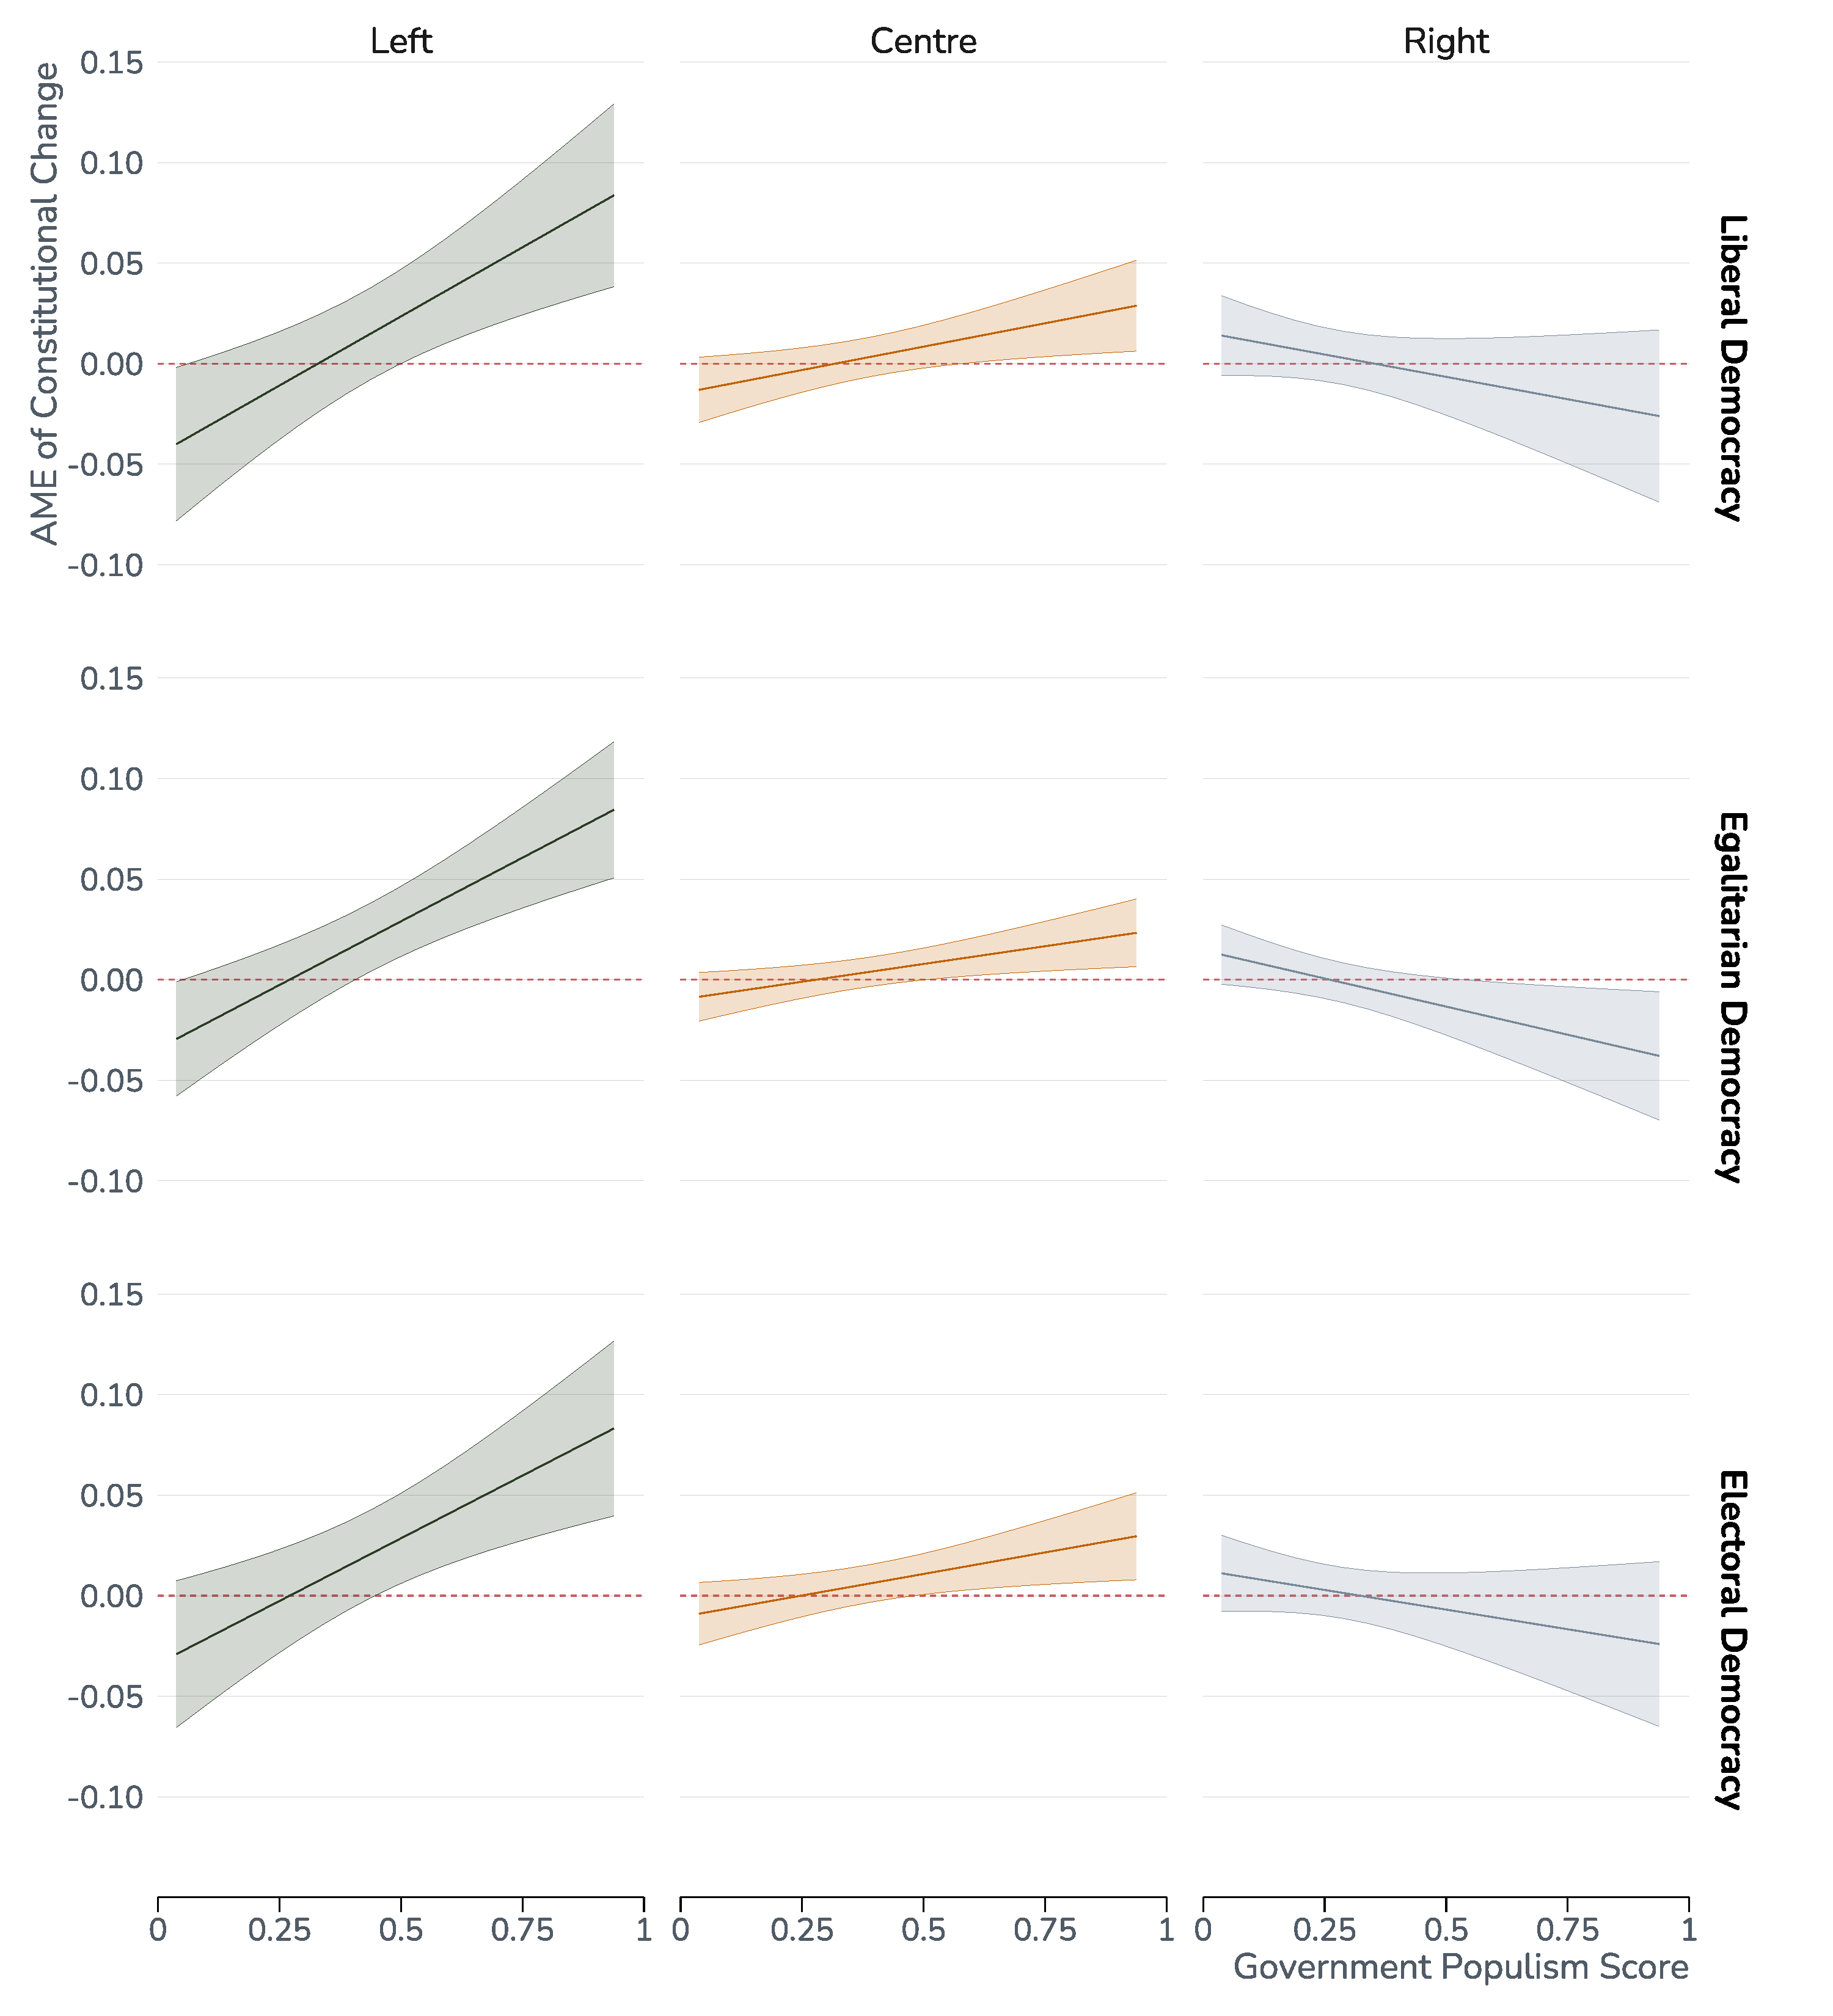
\includegraphics{results/graphs/change_effect.pdf}

}

\caption{\label{fig-interaction}Average marginal effect of
constitutional change conditioned by government ideology and government
populism score.}

\end{figure}

\hypertarget{alternative-explanations}{%
\subsubsection{Alternative
Explanations}\label{alternative-explanations}}

\textbf{Dynamic Models}

As argued before, the effect of populists in power on democratic quality
can also depend on how a democracy has developed before populists came
into power or implemented constitutional changes. In a democracy that is
very elitist, populists can have a more positive impact on participation
than in a democracy where citizens already have a wide range of
possibilities to engage (Mudde \& Rovira Kaltwasser, 2012a, 2017). In
the case of liberal democracy and polyarchy, younger institutions are
more volatile to threats since they still need to build up there
legitimacy (Ruth--Lovell \& Grahn, 2023; \textbf{Gibler.2011?})

We test whether this has an impact on our results by replacing the
ideology dummy with the democratic quality ahead of the respective
country-year observation. We now interact the populism score,
constitutional changes and the lag (2) of the dependent democracy
dimension. Table~\ref{tbl-dynamic} in the appendix shows that the
triple-interaction effect is not significant in most models. Only in the
case of the quality of civil society do we find that the effect differs
depending on the quality before the observation. In countries that have
had a lower quality of civil society, populists in government have a
stronger negative effect on the former (see appendix
Figure~\ref{fig-dynamic}). However, the robustness check does not show
any results that imply that the former quality of democracy drives the
significant results in our main models on the dimensions of liberal
democracy, polyarchy and egalitarianism.

\textbf{Measuring Changes in Constitutional Rights}

Our research design has some limitations. We do not analyze the content
of constitutional changes itself, we only use the change in democratic
quality after a constitutional change. This leaves the possibility that
populist governments implement the expected changes in the constitution,
such as limitations on checks and balances or participation mechanisms,
but that these do not have an effect on the quality of democracy. We try
to answer this data by building indices on rights for the executive and
the judiciary, political and social rights based on the CCP
data.\footnote{The strength of the executive is measured by an index
  developed by Melton \& Ginsburg (2014). This measures whether the
  executive has the power to initiate legislation or constitutional
  amendments, issue decrees, declare a state of emergency, as well as
  enforce its power over other institutions through veto power, and have
  rights reviewed for constitutionality or dissolve parliament. The
  index of independent judiciary rights is based on Melton \& Ginsburg
  (2014) and measures the number of constitutional norms that strengthen
  an independent judiciary (Included are the independence of the
  judiciary in the constitution, whether at least two actors are
  involved in the nomination and appointment of judges to the
  Constitutional Court, whether the dismissal of judges is severely
  restricted and limited only to serious misconduct or constitutional
  violations, and whether judges' salaries are protected. Instead of
  including lifetime appointments, we include whether the re-election of
  judges is excluded.) The index of political rights includes the
  guarantee of freedom of expression, as well as freedom of assembly,
  science, press, strike and trade union rights. Social rights include
  the guarantee of a certain standard of living, health protection at
  work, financial support, social security, and the right to a fair
  trial.}

The indices on executive and judicial power only show any changes in 6
out of 84 cases with a populism score \textgreater{} 0.5. In these
cases, the data shows an increase in executive rights and a decrease in
rights for the judiciary (see Figure~\ref{fig-rightschange}). However, a
very large majority of constitutional changes under populist governments
did not aggrandize power.\footnote{We test whether this relationship is
  significant in a regression model shown in the appendix,
  Table~\ref{tbl-executive}. The results show that even if a populist
  government has a large share of surplus seats, there is no increased
  likelihood of an increase in rights for the executive (see appendix
  Figure~\ref{fig-executive}).}

\begin{figure}

{\centering 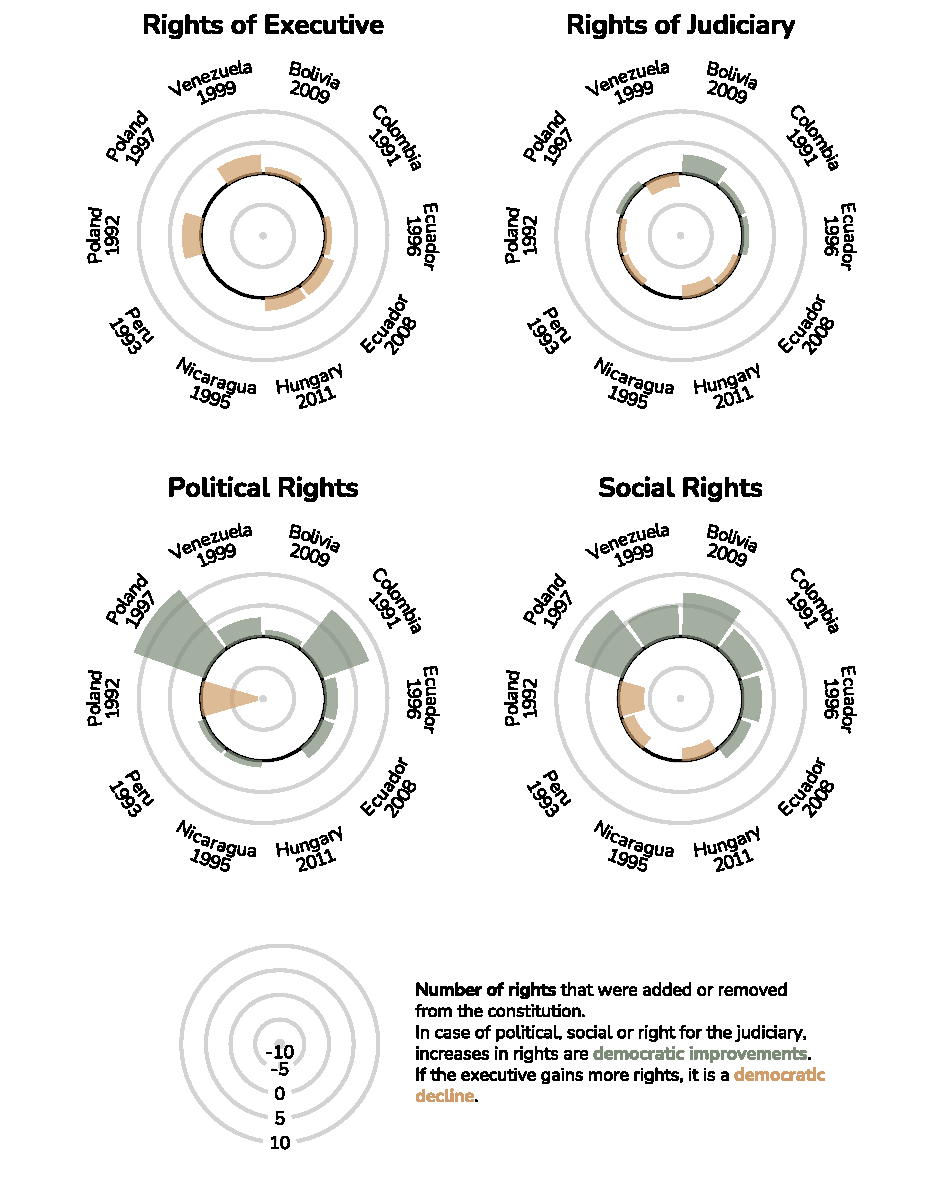
\includegraphics[width=1\textwidth,height=\textheight]{results/graphs/rights_change.pdf}

}

\caption{\label{fig-rightschange}Content changes of constitutional
amendments by populist governments (government weighted populism score
\textgreater{} 0.5) that led to democratic regression.}

\end{figure}

Considering social and political rights, we see a mixed picture. Some
populist governments seem to have increased political and social rights,
while in other cases particularly social rights were decreased (see
Figure~\ref{fig-rightschange}). But, the indices only show differences
for 9 out of the 84 cases with a populism score \textgreater{} 0.5.
While the data corroborates the argument that not all populist parties
in power act in the same way, the small number of cases in which we can
measure a change in written constitutional rights, does not allow for
any inferences to all populist governments.

\hypertarget{conclusion}{%
\subsection{CONCLUSION}\label{conclusion}}

To our knowledge, this is one of the first papers that evaluates the
impact of constitutional changes under populist governments in a large-N
analysis. Our findings confirm the warnings against drawing too quick
conclusions about the relationship between populism and constitutional
change (Blokker et al., 2019; Tushnet \& Bugarič, 2021). We can neither
find support for the arguments that populists frequently adapt the
constitution to the will of the majority(Tushnet \& Bugarič, 2021),
neither do we observe that populists use such changes to aggrandize
power (Mudde, 2021; Müller, 2017a).

Instead, our results show that left-wing populists have even had a
positive effect on liberal democracy, polyarchy and egalitarianism
through their constitutional changes. Constitutional reforms under
right-wing populist governments only had a negative effect on the
quality of egalitarianism. However, we do not find that constitutional
changes under populist governments significantly affect the quality of
participation and civil society.

On the one hand, our results are in contrast with the thesis that
populists in governments use constitutional changes to undermine liberal
democracy (Arato, 2019; Mudde, 2021; Müller, 2017a; Scheppele, 2019). On
the other hand, they corroborate the calls of scholars to regard
populism as a heterogeneous phenomenon that is not necessarily bad for
all aspects of democracy (Blokker et al., 2019; Mudde \& Rovira
Kaltwasser, 2012b, 2013). Both, our analysis as well as the description
of what rights were changed under populist governments show that there
is a heterogeneity between populist parties. Not all populists are the
same.

Considering the relationship between constitutionalism and populism, we
argue that our results have two main implications: Our understanding of
constitutional changes under populist governments are too informed by
few salient cases, such as Hungary. Once we look at the bigger picture,
we do not find the expected negative effect on liberal democratic
institutions and polyarchy. Neither do we find the positive effect on
participation that we have observed in some countries, such as Bolivia,
on a large scale.

Our research further implies that we often overestimate the role that
constitutions play for populists (Blokker, 2019c; Mudde, 2021; Müller,
2017a). We do not find any evidence for arguments that view populists as
proponents of judicial populism (Blokker, 2019c; Tushnet \& Bugarič,
2021). Neither did populists adapt the constitution more often which
could have shown a frequent adaptation to the public's interests, nor do
they improve participation through their constitutional changes.

Future research should consider in more detail how constitutional texts
are changed and how populist voters view such changes. Further, the
support for citizens for such changes is crucial in constitutional
democracies (Engst \& Gschwend, 2023). But, so far, we know very little
about how voters perceive constitutional changes under populist
governments (Magalhães \& Garoupa, 2023). This paper provides some
evidence on how populist parties use constitutional changes once they
are in power. Our approach to compare a 57 countries across two
continents shows that we need to look beyond well known cases because
populists use constitutional changes in variety of ways. We hope that
others follow and more research on the complex relationship between
populism and constitutionalism will follow.

\hypertarget{references}{%
\subsubsection{References}\label{references}}

\hypertarget{refs}{}
\begin{CSLReferences}{1}{0}
\leavevmode\vadjust pre{\hypertarget{ref-Abts.2007}{}}%
Abts, K. \& Rummens, S. (2007).
\href{https://doi.org/10.1111/j.1467-9248.2007.00657.x}{Populism versus
democracy}. \emph{Political Studies} \emph{55}(2): 405--424.

\leavevmode\vadjust pre{\hypertarget{ref-Angelucci.2024}{}}%
Angelucci, D., Rojon, S. \& Vittori, D. (2024).
\href{https://doi.org/10.1080/13569775.2023.2296748}{Do populist parties
promote direct democracy? An empirical assessment in 29 countries in the
last two decades}. \emph{Contemporary Politics} 1--21.

\leavevmode\vadjust pre{\hypertarget{ref-Arato.2019}{}}%
Arato, A. (2019). Populism, constitutional court and civil society. In
C. Landfried (ed.), \emph{Judicial power}. Cambridge, United Kingdom;
New York, NY: {Cambridge University Press}.

\leavevmode\vadjust pre{\hypertarget{ref-AydinCakir.2023}{}}%
Aydin-Cakir, A. (2023).
\href{https://doi.org/10.1080/13501763.2023.2171089}{The varying effect
of court-curbing: Evidence from hungary and poland}. \emph{Journal of
European Public Policy} 1--27.

\leavevmode\vadjust pre{\hypertarget{ref-Blokker.2019c}{}}%
Blokker, P. (2019a). Populist constitutionalism. In C. de La Torre
(ed.), \emph{Routledge handbook of global populism}. London; New York:
Routledge.

\leavevmode\vadjust pre{\hypertarget{ref-Blokker.2019d}{}}%
Blokker, P. (2019b). Varieties of populist constitutionalism: The
transnational dimension. \emph{German Law Journal} \emph{20}(3):
332--350. Retrieved from
\url{https://www.cambridge.org/core/journals/german-law-journal/article/varieties-of-populist-constitutionalism-the-transnational-dimension/4D1C7CC74BD867FEF99D9FD9C078382A}

\leavevmode\vadjust pre{\hypertarget{ref-Blokker.2019e}{}}%
Blokker, P. (2019c). \href{https://doi.org/10.1093/icon/moz028}{Populism
as a constitutional project}. \emph{International Journal of
Constitutional Law} \emph{17}(2): 536--553.

\leavevmode\vadjust pre{\hypertarget{ref-Blokker.2020d}{}}%
Blokker, P. (2020). Populism and constitutional reform. The case of
italy. In G. Delledonne, G. Martinico, M. Monti \& F. Pacini (eds.),
\emph{Italian populism and constitutional law}. Cham: {Palgrave
Macmillan}.

\leavevmode\vadjust pre{\hypertarget{ref-Blokker.2019b}{}}%
Blokker, P., Bugaric, B. \& Halmai, G. (2019).
\href{https://doi.org/10.1017/glj.2019.24}{Introduction: Populist
constitutionalism: Varieties, complexities, and contradictions}.
\emph{German Law Journal} \emph{20}(3): 291--295.

\leavevmode\vadjust pre{\hypertarget{ref-Canovan.1999}{}}%
Canovan, M. (1999). \href{https://doi.org/10.1111/1467-9248.00184}{Trust
the people! Populism and the two faces of democracy}. \emph{Political
Studies} \emph{47}(1): 2--16.

\leavevmode\vadjust pre{\hypertarget{ref-vdemdata.2022}{}}%
Coppedge, M., John Gerring, Carl Henrik Knutsen, C.H., Staffan I.
Lindberg, S., Jan Teorell, J., Nazifa Alizada, N., \ldots{} Daniel
Ziblatt. (2022). V- dem country--year dataset v12: Varieties of
democracy (v-dem) project. {Varieties of Democracy (V-Dem) Project}.

\leavevmode\vadjust pre{\hypertarget{ref-Vdem.2021}{}}%
Coppedge, M., John Gerring, Carl Henrik Knutsen, Staffan I. Lindberg,
Jan Teorell, Nazifa Alizada, \ldots{} Daniel Ziblatt. (2021).
\href{https://doi.org/10.23696/VDEMDS21}{V-dem dataset 2021. Varieties
of democracy (v-dem) project}. {Varieties of Democracy (V-Dem) Project}.

\leavevmode\vadjust pre{\hypertarget{ref-LaTorre.2020}{}}%
de La Torre, C. \& de Lara, F.B. (2020).
\href{https://doi.org/10.1285/I20356609V13I3P1453}{Populism,
constitution making, and the rule of law in latin america}.
\emph{Partecipazione e conflitto,} \emph{13}(3): 1453--1468.

\leavevmode\vadjust pre{\hypertarget{ref-LaTorre.2018}{}}%
de La Torre, C. \& Peruzzotti, E. (2018).
\href{https://doi.org/10.1163/25888072-01011002}{Populism in power:
Between inclusion and autocracy}. \emph{Populism} \emph{1}(1): 38--58.

\leavevmode\vadjust pre{\hypertarget{ref-ComparativeConstitutions.2005}{}}%
Elkins, Z., Ginsburg, T. \& Melton, J. (2021). Characteristics of
national constitutions, version 3.0. Comparative constitutions project.
Retrieved from
\href{https://comparativeconstitutionsproject.org}{comparativeconstitutionsproject.org}

\leavevmode\vadjust pre{\hypertarget{ref-Engst.2023}{}}%
Engst, B. \& Gschwend, T. (2023). Citizens' commitment to judicial
independence: A discrete choice experiment in nine european countries.
Working paper. Retrieved from
\url{https://www.sowi.uni-mannheim.de/media/Lehrstuehle/sowi/Gschwend/Articel/Paper_DCE-EU.pdf}

\leavevmode\vadjust pre{\hypertarget{ref-Fabbrizi.2020}{}}%
Fabbrizi, V. (2020).
\href{https://doi.org/10.1007/s11158-019-09430-7}{Constitutional
democracy in the age of populisms: A commentary to mark tushnet's
populist constitutional law}. \emph{Res Publica} \emph{26}(3): 433--449.

\leavevmode\vadjust pre{\hypertarget{ref-Gherghina.2021b}{}}%
Gherghina, S. \& Pilet, J.-B. (2021). Do populist parties support
referendums? A comparative analysis of election manifestos in europe.
\emph{Electoral Studies} \emph{74}: 102419. Retrieved from
\url{https://www.sciencedirect.com/science/article/pii/S0261379421001311}

\leavevmode\vadjust pre{\hypertarget{ref-Haas.2022}{}}%
Haas, V. (n.d.). Changing the rules of the game? Populists in power and
constitutional retrogression {[}paper presentation{]}. EPSA 2022:
European political science association, prague, czech republic.
Retrieved from \url{https://violeta-haas.github.io/research/}

\leavevmode\vadjust pre{\hypertarget{ref-Habermas.2001}{}}%
Habermas, J. \& Rehg, W. (2001). Constitutional democracy: A paradoxical
union of contradictory principles? \emph{Political Theory} \emph{29}(6):
766--781.

\leavevmode\vadjust pre{\hypertarget{ref-Hilgers.2013}{}}%
Hilgers, T. (2013). \emph{Clientelism in everyday latin american
politics}. New York: {Palgrave Macmillan}.

\leavevmode\vadjust pre{\hypertarget{ref-Houle.2018}{}}%
Houle, C. \& Kenny, P.D. (2018).
\href{https://doi.org/10.1017/gov.2016.25}{The political and economic
consequences of populist rule in latin america}. \emph{Government and
Opposition} \emph{53}(2): 256--287.

\leavevmode\vadjust pre{\hypertarget{ref-Huber.2022}{}}%
Huber, R.A., Jankowski, M. \& JUEN, C. (2022).
\href{https://doi.org/10.1111/1475-6765.12569}{Populist parties and the
two--dimensional policy space}. \emph{European Journal of Political
Research}.

\leavevmode\vadjust pre{\hypertarget{ref-Huber.2017}{}}%
Huber, R.A. \& Schimpf, C.H. (2017).
\href{https://doi.org/10.17645/pag.v5i4.919}{On the distinct effects of
left-wing and right-wing populism on democratic quality}. \emph{Politics
and Governance} \emph{5}(4): 146--165.

\leavevmode\vadjust pre{\hypertarget{ref-Huq.2018}{}}%
Huq, A. \& Ginsburg, T. (2018). How to lose a constitutional democracy.
\emph{UCLA Law Review} \emph{65}: 78. Retrieved from
\url{https://heinonline.org/HOL/Page?handle=hein.journals/uclalr65\&id=88\&div=\&collection=}

\leavevmode\vadjust pre{\hypertarget{ref-Jolly.2022}{}}%
Jolly, S., Bakker, R., Hooghe, L., Marks, G., Polk, J., Rovny, J.,
\ldots{} Vachudova, M.A. (2022).
\href{https://doi.org/10.1016/j.electstud.2021.102420}{Chapel hill
expert survey trend file, 1999--2019}. \emph{Electoral Studies}
\emph{75}: 102420.

\leavevmode\vadjust pre{\hypertarget{ref-Kenny.2020}{}}%
Kenny, P.D. (2020).
\href{https://doi.org/10.1177/1065912918824038}{{`The enemy of the
people'}: Populists and press freedom}. \emph{Political Research
Quarterly} \emph{73}(2): 261--275.

\leavevmode\vadjust pre{\hypertarget{ref-Konig.2023b}{}}%
König, J.S. \& Swalve, T. (n.d.). Zum verh{ä}ltnis von demokratischer
und konstitutioneller regression unter populistischen regierungen - eine
empirische analyse. \emph{Leviathan} \emph{Sonderband}(40). Retrieved
from
\url{https://www.nomos-shop.de/nomos/titel/zur-diagnose-demokratischer-regression-id-105862/}

\leavevmode\vadjust pre{\hypertarget{ref-Lacey.2019}{}}%
Lacey, N. (2019). Populism and the rule of law. \emph{Annual Review of
Law and Social Science} \emph{15}: 79--96.

\leavevmode\vadjust pre{\hypertarget{ref-Laclau.2005}{}}%
Laclau, E. (2005). \emph{On populist reason}. London: Verso.

\leavevmode\vadjust pre{\hypertarget{ref-Landau.2013}{}}%
Landau, D. (2013). Abusive constitutionalism. \emph{UC Davis Law Review}
\emph{47}(1): 189--260.

\leavevmode\vadjust pre{\hypertarget{ref-VParty.2022}{}}%
Lindberg, S., Nils Düpont, Masaaki Higashijima, Yaman Berker Kavasoglu,
Kyle L. Marquardt, Michael Bernhard, \ldots{} Brigitte Seim. (2022).
\href{https://doi.org/10.23696/VPARTYDSV2}{Varieties of party identity
and organization (v--party) dataset V2. Varieties of democracy (v-dem)
project.} {V-Dem Institute}.

\leavevmode\vadjust pre{\hypertarget{ref-VParty.2020}{}}%
Lührmann, A., Nils Düpont, Masaaki Higashijima, Yaman Berker Kavasoglu,
Kyle L. Marquardt, Michael Bernhard, \ldots{} Brigitte Seim. (2020).
\href{https://doi.org/10.23696/VPARTYDSV1}{V-party dataset V1}.
(Varieties of Democracy (V-Dem) Project, ed.). {V-Dem Institute}.

\leavevmode\vadjust pre{\hypertarget{ref-Magalhaes.2023}{}}%
Magalhães, P.C. \& Garoupa, N. (2023).
\href{https://doi.org/10.1080/13501763.2023.2235386}{Populist
governments, judicial independence, and public trust in the courts}.
\emph{Journal of European Public Policy} 1--28.

\leavevmode\vadjust pre{\hypertarget{ref-MartinezGallardo.2023}{}}%
Martínez-Gallardo, C., La Cerda, N. de, Hartlyn, J., Hooghe, L., Marks,
G. \& Bakker, R. (2023).
\href{https://doi.org/10.1177/13540688221090604}{Revisiting party system
structuration in latin america and europe: Economic and socio-cultural
dimensions}. \emph{Party Politics} \emph{29}(4): 780--792.

\leavevmode\vadjust pre{\hypertarget{ref-Mastropaolo.2021}{}}%
Mastropaolo, A. (2021). Populism and political representation. In R.
Heinisch, C. Holtz-Bacha \& O. Mazzoleni (eds.), \emph{Political
populism}. {[}S.l.{]}: {Nomos Verlagsgesellschaft}.

\leavevmode\vadjust pre{\hypertarget{ref-Mazzoleni.2020}{}}%
Mazzoleni, O. \& Voerman, G. (2020).
\href{https://doi.org/10.1285/I20356609V13I3P1417}{In the name of
sovereignty. Right-wing populism and the power of the judiciary in
western europe}. \emph{Partecipazione e conflitto} \emph{13}(3):
1417--1432.

\leavevmode\vadjust pre{\hypertarget{ref-Melton.2014}{}}%
Melton, J. \& Ginsburg, T. (2014). Does de jure judicial independence
really matter: A reevaluation of explanations for judicial independence.
\emph{Journal of Law and Courts} \emph{2}(2): 187--217. Retrieved from
\url{https://heinonline.org/HOL/Page?handle=hein.journals/jlawct2\&id=187\&div=11\&collection=journals}

\leavevmode\vadjust pre{\hypertarget{ref-Meny.2002b}{}}%
Mény, Y. \& Surel, Y. (2002). The constitutive ambiguity of populism. In
Y. Mény \& Y. Surel (eds.), \emph{Democracies and the populist
challenge}. Basingstoke, Hampshire; New York: Palgrave.

\leavevmode\vadjust pre{\hypertarget{ref-Mouffe.2005}{}}%
Mouffe, C. (2005). \emph{On the political}. London: Routledge.

\leavevmode\vadjust pre{\hypertarget{ref-Mudde.2004}{}}%
Mudde, C. (2004).
\href{https://doi.org/10.1111/j.1477-7053.2004.00135.x}{The populist
zeitgeist}. \emph{Government and Opposition} \emph{39}(4): 541--563.

\leavevmode\vadjust pre{\hypertarget{ref-Mudde.2021}{}}%
Mudde, C. (2021). Populism and constitutionalism. In N. Holtug \& E. M.
Uslaner (eds.), \emph{National identity and social cohesion}. London;
New York: {ecpr Press Rowman {\&} Littlefield}.

\leavevmode\vadjust pre{\hypertarget{ref-Mudde.2012}{}}%
Mudde, C. \& Rovira Kaltwasser, C. (2012a). Populism and (liberal)
democracy: A framework for analysis. In C. Mudde \& C. Rovira Kaltwasser
(eds.), \emph{Populism in europe and the americas}. Cambridge; New York:
{Cambridge University Press}.

\leavevmode\vadjust pre{\hypertarget{ref-Mudde.2012b}{}}%
Mudde, C. \& Rovira Kaltwasser, C. (2012b). Populism: Corrective and
threat to democracy. In C. Mudde \& C. Rovira Kaltwasser (eds.),
\emph{Populism in europe and the americas}. Cambridge; New York:
{Cambridge University Press}.

\leavevmode\vadjust pre{\hypertarget{ref-Mudde.2013b}{}}%
Mudde, C. \& Rovira Kaltwasser, C. (2013).
\href{https://doi.org/10.1017/gov.2012.11}{Exclusionary vs. Inclusionary
populism: Comparing contemporary europe and latin america}.
\emph{Government and Opposition} \emph{48}(2): 147--174.

\leavevmode\vadjust pre{\hypertarget{ref-Mudde.2017b}{}}%
Mudde, C. \& Rovira Kaltwasser, C. (2017). \emph{Populism: A very short
introduction}. Oxford; New York, NY: {Oxford University Press}.

\leavevmode\vadjust pre{\hypertarget{ref-Muller.2016}{}}%
Müller, J.-W. (2016). \emph{What is populism?} Philadelphia: {University
of Pennsylvania Press Inc}.

\leavevmode\vadjust pre{\hypertarget{ref-Muller.2017}{}}%
Müller, J.-W. (2017a). Populism and constitutionalism. In C. Rovira
Kaltwasser, P. A. Taggart, P. Ochoa Espejo \& P. Ostiguy (eds.),
\emph{The oxford handbook of populism}. Oxford; New York: {Oxford
University Press}.

\leavevmode\vadjust pre{\hypertarget{ref-Muller.2017b}{}}%
Müller, J.-W. (2017b). \emph{Was ist populismus? Ein essay}
(Originalausgabe, 5. Auflage 2017.). Berlin: {Suhrkamp Verlag};
Suhrkamp.

\leavevmode\vadjust pre{\hypertarget{ref-CristobalRoviraKaltwasser.2013}{}}%
Rovira Kaltwasser, C. (2013). Populism vs. Constitutionalism?
Comparative perspectives on contemporary western europe, latin america,
and the united states. {The Foundation for Law, Justice and Society}.
Retrieved from
\url{https://ora.ox.ac.uk/objects/uuid:0b3a92d0-401b-4af8-a4bd-89afb98e7454}

\leavevmode\vadjust pre{\hypertarget{ref-Ruth.2018}{}}%
Ruth, S.P. (2018).
\href{https://doi.org/10.1177/0032321717723511}{Populism and the erosion
of horizontal accountability in latin america}. \emph{Political Studies}
\emph{66}(2): 356--375.

\leavevmode\vadjust pre{\hypertarget{ref-RuthLovell.2022}{}}%
Ruth--Lovell, S.P. \& Grahn, S. (2023).
\href{https://doi.org/10.1111/1475-6765.12564}{Threat or corrective to
democracy? The relationship between populism and different models of
democracy}. \emph{European Journal of Political Research} \emph{62}(3):
677--698.

\leavevmode\vadjust pre{\hypertarget{ref-Scheppele.2018}{}}%
Scheppele, K.L. (2018). Autocratic legalism. \emph{The University of
Chicago Law Review} \emph{85}(2): 545--584.

\leavevmode\vadjust pre{\hypertarget{ref-Scheppele.2019}{}}%
Scheppele, K.L. (2019). The opportunism of populists and the defense of
constitutional liberalism. \emph{German Law Journal} \emph{20}(3):
314--331. Retrieved from
\url{https://www.cambridge.org/core/journals/german-law-journal/article/opportunism-of-populists-and-the-defense-of-constitutional-liberalism/687EC99BB43AB8AE88FAA42ED4D83DB0}

\leavevmode\vadjust pre{\hypertarget{ref-StoneSweet.2002}{}}%
Stone Sweet, A. (2002). \emph{Governing with judges: Constitutional
politics in europe} (Repr.). Oxford: {Oxford Univ. Press}.

\leavevmode\vadjust pre{\hypertarget{ref-Tushnet.2000}{}}%
Tushnet, M. (2000).
\emph{\href{https://doi.org/10.1515/9781400822973}{Taking the
constitution away from the courts}}. Princeton: {Princeton University
Press}.

\leavevmode\vadjust pre{\hypertarget{ref-Tushnet.2020}{}}%
Tushnet, M. \& Bugaric, B. (2020). Populism and constitutionalism: An
essay on definitions and their implications. Retrieved from
\url{http://nrs.harvard.edu/urn-3:HUL.InstRepos:42660123}

\leavevmode\vadjust pre{\hypertarget{ref-Tushnet.2021}{}}%
Tushnet, M. \& Bugarič, B. (2021).
\emph{\href{https://doi.org/10.1093/oso/9780197606711.001.0001}{Power to
the people: Constitutionalism in the age of populism}}. New York, NY:
{Oxford University Press}.

\leavevmode\vadjust pre{\hypertarget{ref-Vittori.2022}{}}%
Vittori, D. (2022). Threat or corrective? Assessing the impact of
populist parties in government on the qualities of democracy: A
19-country comparison. \emph{Government and Opposition} \emph{57}(4):
589--609. Retrieved from
\url{https://www.cambridge.org/core/journals/government-and-opposition/article/threat-or-corrective-assessing-the-impact-of-populist-parties-in-government-on-the-qualities-of-democracy-a-19country-comparison/BDCB69DB98745BC6CA5961586C76B010}

\leavevmode\vadjust pre{\hypertarget{ref-Waldron.2006}{}}%
Waldron, J. (2006). The core of the case against judicial review.
\emph{Yale Law Journal} \emph{115}(6): 1346. Retrieved from
\url{http://www.jstor.org/stable/20455656}

\leavevmode\vadjust pre{\hypertarget{ref-Waldron.2021}{}}%
Waldron, J. (2021). The rule of law and the role of courts. \emph{Global
Constitutionalism} \emph{10}(1): 91--105. Retrieved from
\url{https://www.cambridge.org/core/journals/global-constitutionalism/article/rule-of-law-and-the-role-of-courts/2E4BC01A2170132CBEEE8ACCB509DC11}

\leavevmode\vadjust pre{\hypertarget{ref-Whittington.2010}{}}%
Whittington, K.E. (2010). Constitutionalism. In K. E. Whittington, R. D.
Kelemen \& G. A. Caldeira (eds.), \emph{The oxford handbook of law and
politics}. Oxford: {Oxford Univ. Pr}.

\end{CSLReferences}

\newpage{}

\hypertarget{appendix-constitutional-changes}{%
\subsection{APPENDIX CONSTITUTIONAL
CHANGES}\label{appendix-constitutional-changes}}

\newpage{}

\scriptsize

\hypertarget{tbl-populistchanges}{}
\begin{longtable}{l|lrr}
\caption{\label{tbl-populistchanges}Constitutional changes under populist governments (weighted populism
score \textgreater{} 0.5) }\tabularnewline

\toprule
\multicolumn{1}{l}{} & \textbf{Country} & \textbf{Years} & \textbf{Const. Changes} \\ 
\midrule\addlinespace[2.5pt]
\multicolumn{4}{l}{Latin America} \\ 
\midrule\addlinespace[2.5pt]
 & Bolivia & 2005, 2009 & 2 \\ 
 & Colombia & 1991, 1993, 1995, 1996, 1997 & 5 \\ 
 & Costa Rica & 1991, 1993, 1999, 2000, 2001, 2015, 2018, 2019 & 8 \\ 
 & Ecuador & 1996, 2002, 2008, 2011, 2015, 2018 & 6 \\ 
 & El Salvador & 2009, 2014 & 2 \\ 
 & Guyana & 1992, 1995, 2000 & 3 \\ 
 & Mexico & 2018, 2019 & 2 \\ 
 & Nicaragua & 1994, 1995, 2007, 2010, 2014 & 5 \\ 
 & Paraguay & 2011 & 1 \\ 
 & Peru & 1995, 2002, 2004, 2005, 2015 & 5 \\ 
 & Uruguay & 2004 & 1 \\ 
 & Venezuela & 1999, 2009 & 2 \\ 
\midrule 
Total & — & — & 42 \\ 
\midrule\addlinespace[2.5pt]
\multicolumn{4}{l}{Europe} \\ 
\midrule\addlinespace[2.5pt]
 & Hungary & 1993, 2000, 2001, 2010, 2011, 2012, 2013, 2016, 2018, 2019 & 10 \\ 
 & Latvia & 1991 & 1 \\ 
 & Malta & 1996, 1997, 2000, 2001, 2011, 2014, 2015, 2016, 2018, 2019 & 10 \\ 
 & Poland & 1991, 1992, 1997, 2006 & 4 \\ 
 & Slovakia & 1998, 1999, 2001, 2006, 2012, 2014, 2015 & 7 \\ 
 & Slovenia & 2004, 2006, 2013 & 3 \\ 
 & Switzerland & 2015, 2016, 2017, 2018 & 4 \\ 
 & Ukraine & 2010, 2011, 2019 & 3 \\ 
\midrule 
Total & — & — & 42 \\ 
\bottomrule
\end{longtable}

\blandscape

\hypertarget{tbl-resultschange_EU}{}
\begin{table}
\caption{\label{tbl-resultschange_EU}Regression results for likelihood of constitutional change }\tabularnewline

\centering\centering\centering
\begin{tabular}[t]{lcccc}
\toprule
  & Latin America & GALTAN1 & GALTAN2 & GALTAN3\\
\midrule
Populism & -0.059 & -0.344 & -0.458+ & -2.198+\\
 & {}[-0.318, 0.199] & {}[-0.841, 0.152] & {}[-0.963, 0.046] & {}[-4.593, 0.198]\\
Left-Right & 0.030 &  &  & \\
 & {}[-0.041, 0.101] &  &  & \\
Surplus & 0.000 &  & 0.011* & 0.011*\\
 & {}[-0.005, 0.005] &  & {}[0.001, 0.021] & {}[0.000, 0.021]\\
Coalition & 0.002 &  & -0.075 & -0.097\\
 & {}[-0.101, 0.106] &  & {}[-0.294, 0.144] & {}[-0.317, 0.123]\\
Populism:Left-Right & 0.035 &  &  & \\
 & {}[-0.079, 0.148] &  &  & \\
GAL-TAN &  & 0.021 & 0.013 & -0.082\\
 &  & {}[-0.039, 0.080] & {}[-0.046, 0.073] & {}[-0.224, 0.060]\\
Populism:GAL-TAN &  &  &  & 0.284\\
 &  &  &  & {}[-0.099, 0.667]\\
\midrule
Num.Obs. & 498 & 238 & 238 & 238\\
R2 & 0.027 & 0.009 & 0.030 & 0.039\\
Country FE & Yes & Yes & Yes & Yes\\
R2 Adj. & -0.018 & -0.077 & -0.064 & -0.059\\
AIC & 424.2 & 275.2 & 274.0 & 273.7\\
BIC & 449.5 & 285.6 & 291.4 & 294.5\\
RMSE & 0.37 & 0.43 & 0.42 & 0.42\\
\bottomrule
\multicolumn{5}{l}{\rule{0pt}{1em}+p $<$ 0.1; *p $<$ 0.05; **p > 0.01; ***p $<$ 0.001}\\
\end{tabular}
\end{table}

\hypertarget{tbl-executive}{}
\begin{table}
\caption{\label{tbl-executive}Regression models for changes in rights of the executive }\tabularnewline

\centering\centering\centering
\begin{tabular}[t]{lcccc}
\toprule
  & Base & Controls & Interaction and Controls & Surplus\\
\midrule
Populism & 0.063* & 0.062* & -0.110 & 0.097**\\
 & {}[0.003, 0.123] & {}[0.002, 0.122] & {}[-0.252, 0.032] & {}[0.030, 0.163]\\
Left-Right & 0.009+ & 0.010+ & -0.012 & 0.010+\\
 & {}[-0.001, 0.020] & {}[-0.001, 0.020] & {}[-0.054, 0.030] & {}[0.000, 0.021]\\
Surplus &  & 0.000 & 0.001 & 0.002+\\
 &  & {}[-0.001, 0.001] & {}[-0.002, 0.004] & {}[0.000, 0.004]\\
Coalition &  & -0.003 & 0.015 & -0.004\\
 &  & {}[-0.031, 0.026] & {}[-0.054, 0.084] & {}[-0.032, 0.025]\\
Populism:Left-Right &  &  & 0.077 & \\
 &  &  & {}[-0.017, 0.172] & \\
Populism:Surplus &  &  &  & -0.006*\\
 &  &  &  & {}[-0.011, -0.001]\\
\midrule
Num.Obs. & 1528 & 1528 & 1543 & 1528\\
R2 & 0.004 & 0.004 & 0.008 & 0.007\\
Country FE & Yes & Yes & Yes & Yes\\
R2 Adj. & -0.036 & -0.037 & -0.033 & -0.034\\
AIC & -1115.6 & -1111.6 & 1536.3 & -1115.5\\
BIC & -1099.6 & -1084.9 & 1568.4 & -1083.5\\
RMSE & 0.17 & 0.17 & 0.40 & 0.17\\
\bottomrule
\multicolumn{5}{l}{\rule{0pt}{1em}+p $<$ 0.1; *p $<$ 0.05; **p > 0.01; ***p $<$ 0.001}\\
\end{tabular}
\end{table}

\elandscape

\begin{figure}[H]

{\centering 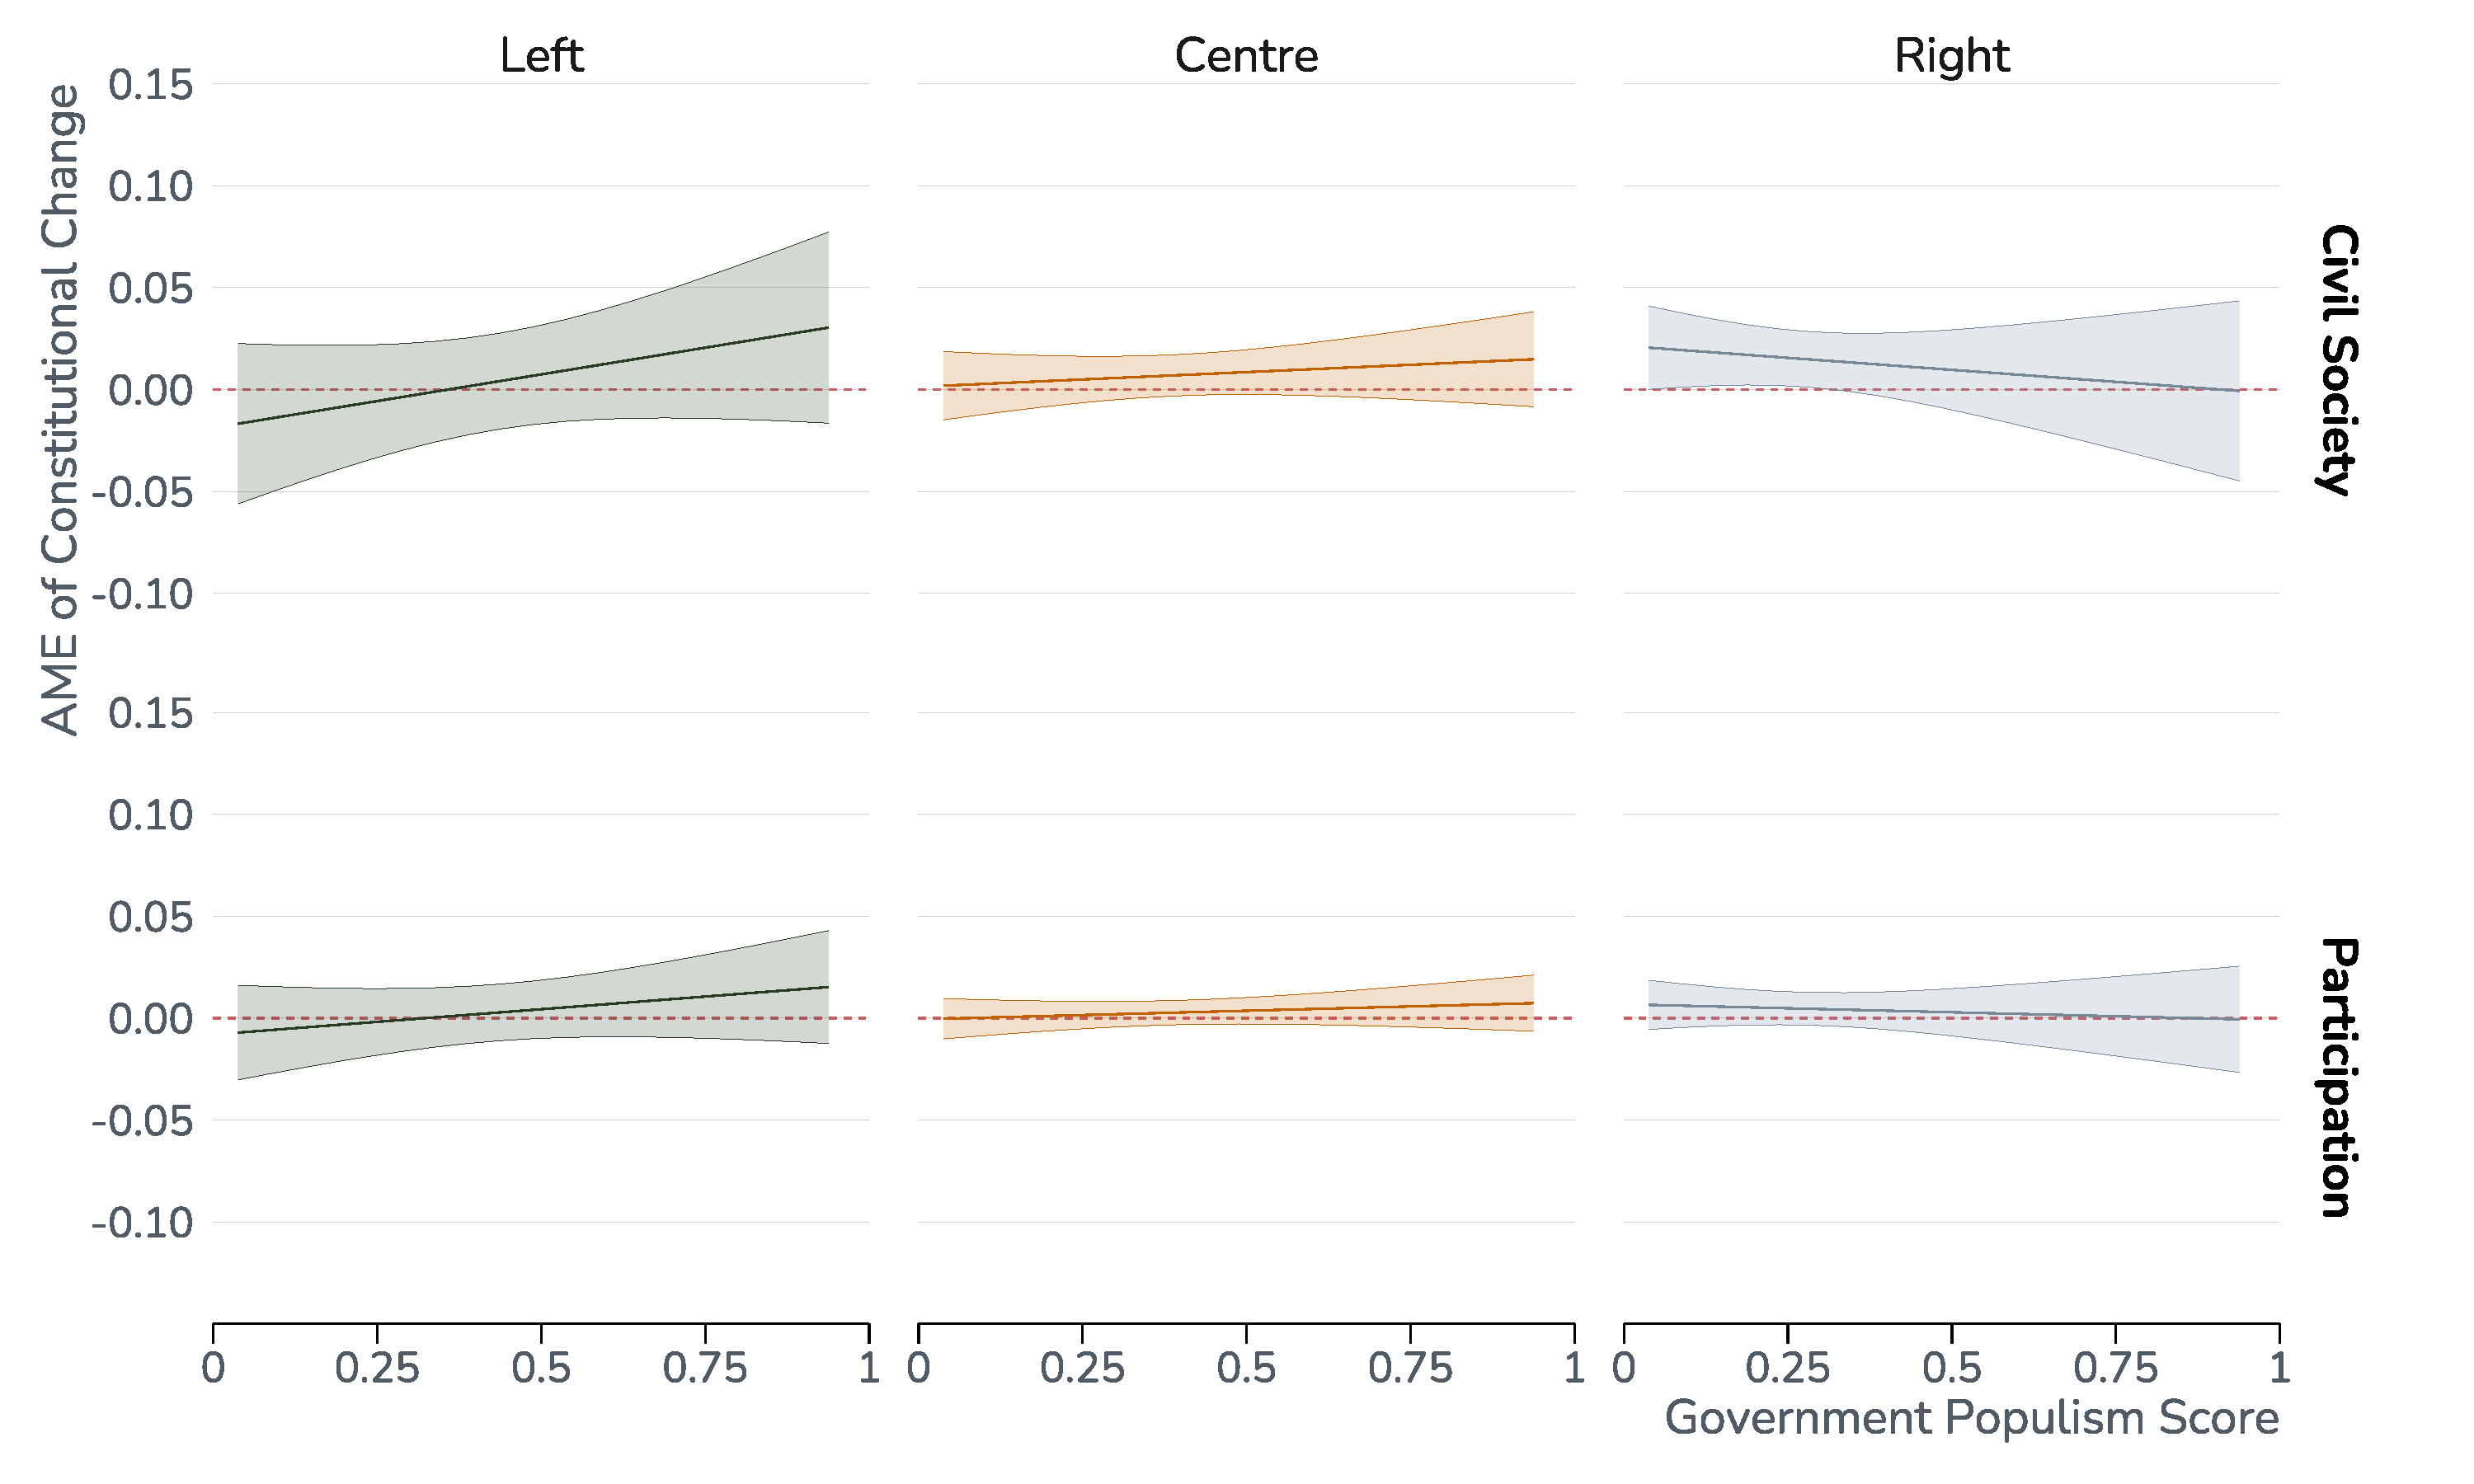
\includegraphics{results/graphs/change_effect_appendix.pdf}

}

\caption{\label{fig-interactionapp}Average marginal effect of
constitutional change condititoned by government weighted populism score
and ideology (based on table \textbf{?@tbl-results}).}

\end{figure}

\begin{figure}[H]

{\centering 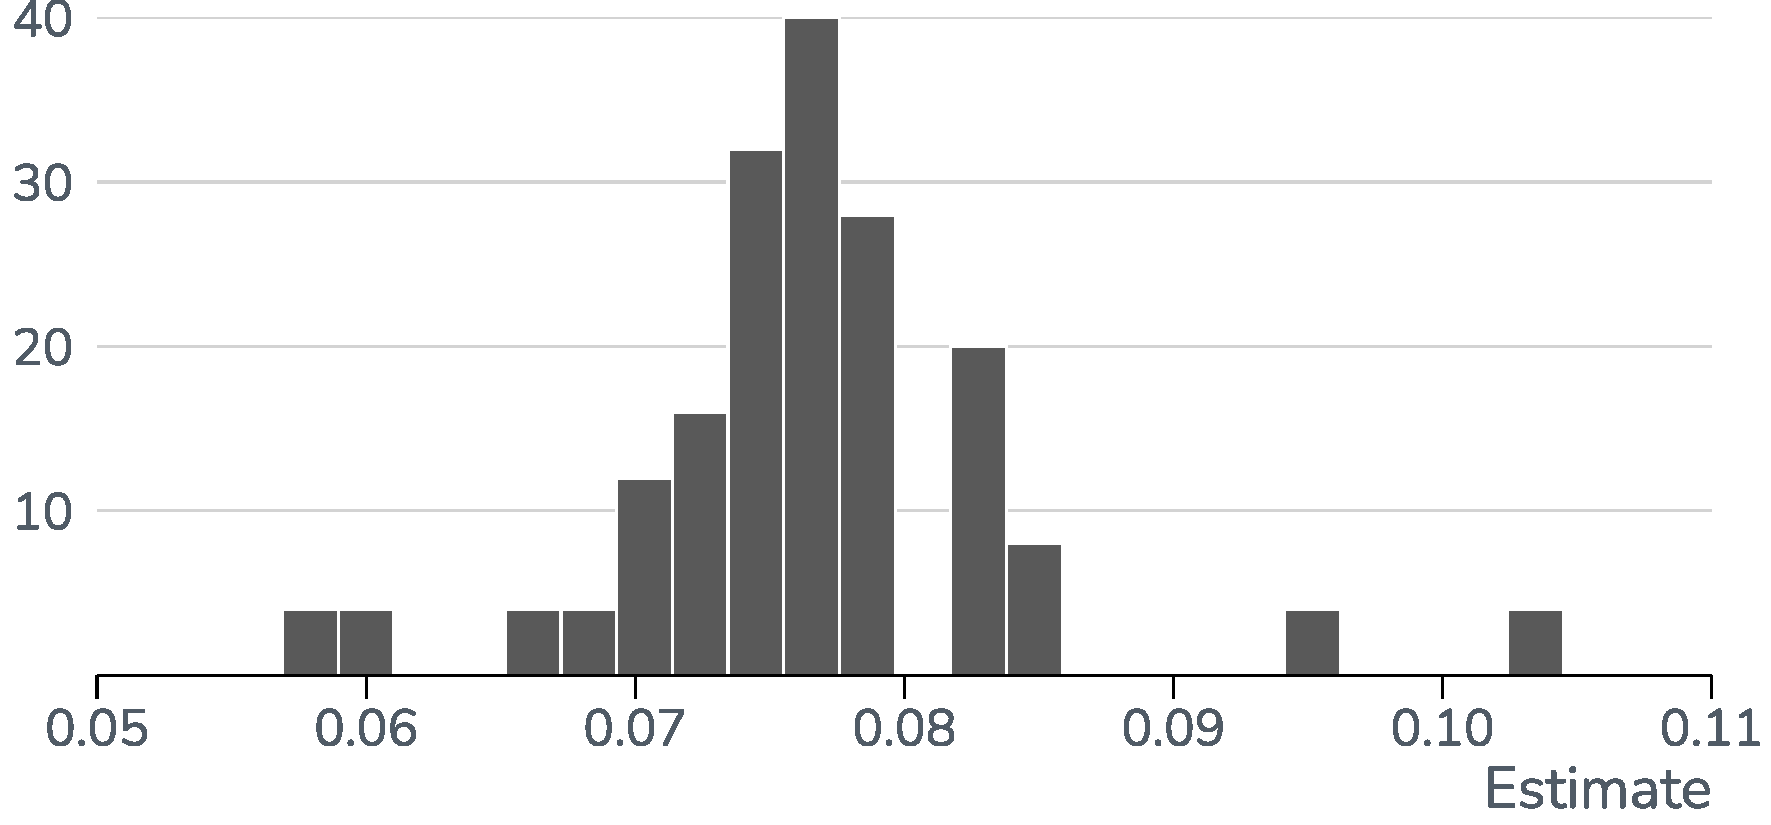
\includegraphics[width=0.9\textwidth,height=\textheight]{results/graphs/jackknife_change.pdf}

}

\caption{\label{fig-jackknifechange}Coefficients of interaction effect
of jackknifed models for \textbf{?@tbl-results}, model 3.}

\end{figure}

\begin{figure}[H]

{\centering 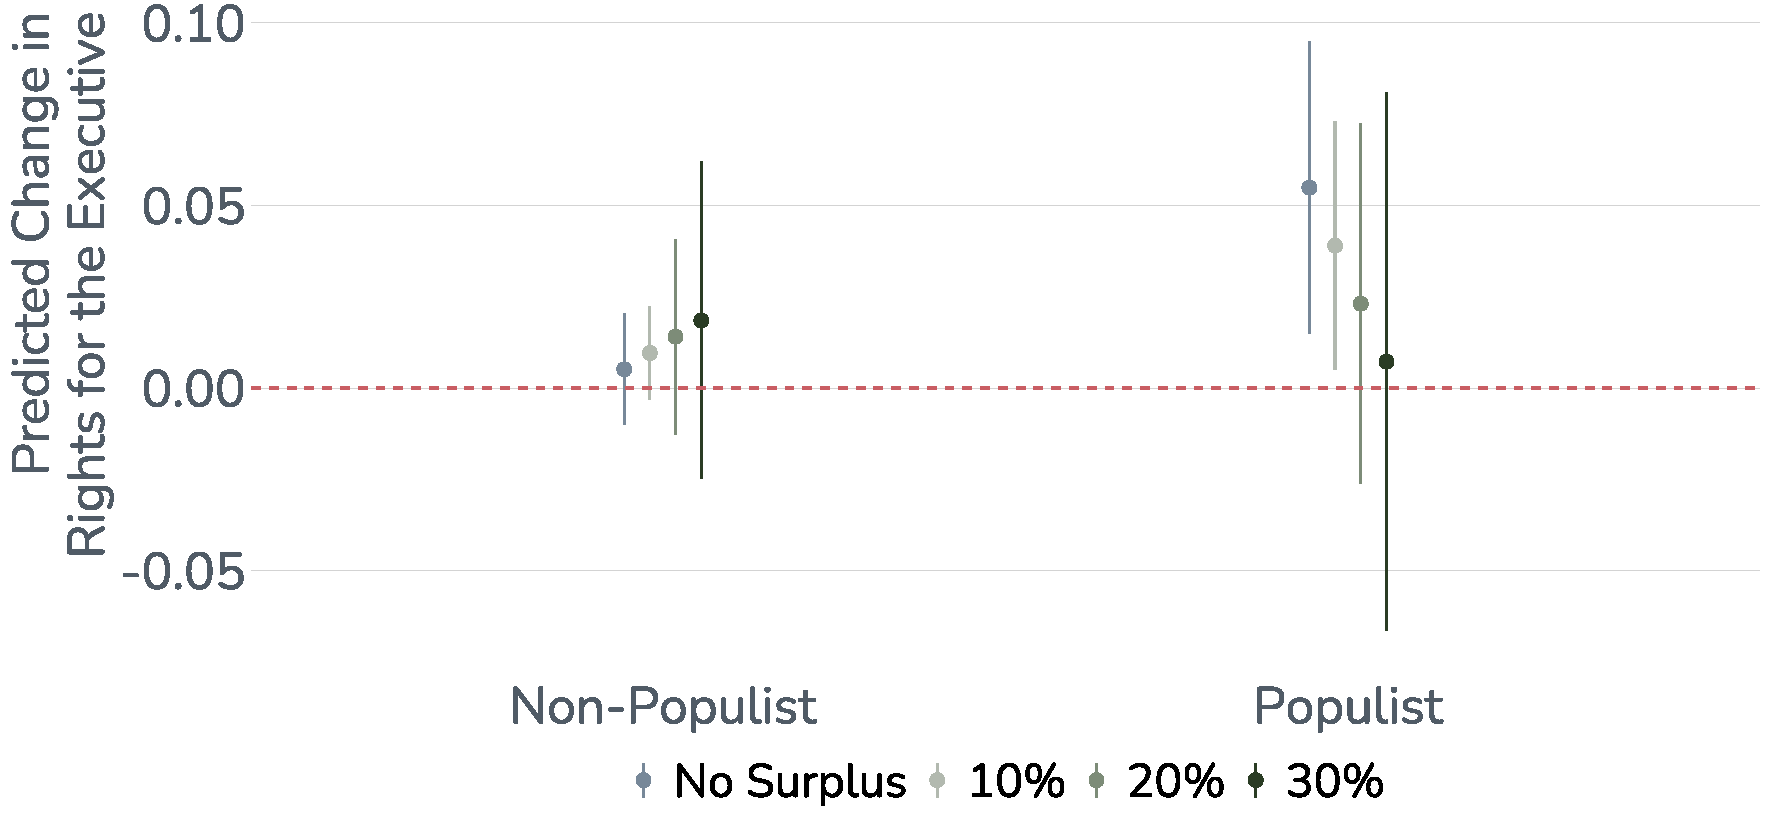
\includegraphics[width=0.9\textwidth,height=\textheight]{results/graphs/change_in_executive.pdf}

}

\caption{\label{fig-executive}Predicted change in rights for the
executive conditioned by ideology and populism based on
Table~\ref{tbl-executive}, model 4.}

\end{figure}

\blandscape
\renewcommand{\arraystretch}{0.5}
\setlength{\tabcolsep}{2pt}

\hypertarget{tbl-libdem}{}
\begin{table}
\caption{\label{tbl-libdem}Full regression models on liberal democracy }\tabularnewline

\centering\centering\centering
\begin{tabular}[t]{lcccccc}
\toprule
  & Populism & Event & Moderator & Controls & Interaction & Triple-Interaction\\
\midrule
Populism & -0.121*** &  &  & -0.111*** & -0.126*** & -0.112***\\
 & {}[-0.142, -0.099] &  &  & {}[-0.133, -0.089] & {}[-0.150, -0.101] & {}[-0.137, -0.086]\\
Const. Change &  & 0.007 &  & 0.004 & -0.010 & -0.009\\
 &  & {}[-0.002, 0.016] &  & {}[-0.004, 0.012] & {}[-0.023, 0.003] & {}[-0.023, 0.006]\\
Left-Right &  &  & 0.006** & -0.007*** & -0.007*** & -0.025***\\
 &  &  & {}[0.002, 0.010] & {}[-0.011, -0.003] & {}[-0.011, -0.003] & {}[-0.032, -0.017]\\
Surplus &  &  &  & -0.003*** & -0.003*** & -0.002***\\
 &  &  &  & {}[-0.003, -0.002] & {}[-0.003, -0.002] & {}[-0.003, -0.002]\\
Coalition &  &  &  & 0.050*** & 0.050*** & 0.043***\\
 &  &  &  & {}[0.039, 0.060] & {}[0.039, 0.060] & {}[0.033, 0.054]\\
Populism:Const. Change &  &  &  &  & 0.046** & 0.028\\
 &  &  &  &  & {}[0.012, 0.079] & {}[-0.008, 0.064]\\
Populism:Left-Right &  &  &  &  &  & 0.050***\\
 &  &  &  &  &  & {}[0.033, 0.066]\\
Const. Change:Left-Right &  &  &  &  &  & 0.013*\\
 &  &  &  &  &  & {}[0.001, 0.025]\\
Populism:Const. Change:Left-Right &  &  &  &  &  & -0.039**\\
 &  &  &  &  &  & {}[-0.064, -0.013]\\
\midrule
Country FE & Yes & Yes & Yes & Yes & Yes & Yes\\
Num.Obs. & 1569 & 1588 & 1569 & 1539 & 1539 & 1539\\
R2 & 0.075 & 0.002 & 0.005 & 0.173 & 0.177 & 0.197\\
R2 Adj. & 0.040 & -0.036 & -0.032 & 0.139 & 0.143 & 0.161\\
AIC & -4017.9 & -3910.0 & -3903.6 & -4159.9 & -4165.3 & -4196.8\\
BIC & -4007.2 & -3899.2 & -3892.9 & -4127.8 & -4127.9 & -4143.4\\
RMSE & 0.07 & 0.07 & 0.07 & 0.06 & 0.06 & 0.06\\
\bottomrule
\multicolumn{7}{l}{\rule{0pt}{1em}+p $<$ 0.1; *p $<$ 0.05; **p > 0.01; ***p $<$ 0.001}\\
\end{tabular}
\end{table}

\renewcommand{\arraystretch}{0.5}
\setlength{\tabcolsep}{2pt}

\hypertarget{tbl-polyarchy}{}
\begin{table}
\caption{\label{tbl-polyarchy}Full regression models on polyarchy }\tabularnewline

\centering\centering\centering
\begin{tabular}[t]{lcccccc}
\toprule
  & Populism & Event & Moderator & Controls & Interaction & Triple-Interaction\\
\midrule
Populism & -0.100*** &  &  & -0.088*** & -0.102*** & -0.087***\\
 & {}[-0.120, -0.079] &  &  & {}[-0.109, -0.066] & {}[-0.126, -0.079] & {}[-0.112, -0.063]\\
Const. Change &  & 0.008+ &  & 0.005 & -0.009 & -0.006\\
 &  & {}[0.000, 0.016] &  & {}[-0.002, 0.013] & {}[-0.022, 0.003] & {}[-0.020, 0.008]\\
Left-Right &  &  & 0.005** & -0.005** & -0.006** & -0.022***\\
 &  &  & {}[0.001, 0.009] & {}[-0.009, -0.002] & {}[-0.010, -0.002] & {}[-0.029, -0.015]\\
Surplus &  &  &  & -0.002*** & -0.002*** & -0.002***\\
 &  &  &  & {}[-0.003, -0.002] & {}[-0.003, -0.002] & {}[-0.003, -0.002]\\
Coalition &  &  &  & 0.046*** & 0.046*** & 0.040***\\
 &  &  &  & {}[0.036, 0.056] & {}[0.036, 0.056] & {}[0.030, 0.050]\\
Populism:Const. Change &  &  &  &  & 0.046** & 0.026\\
 &  &  &  &  & {}[0.014, 0.078] & {}[-0.008, 0.061]\\
Populism:Left-Right &  &  &  &  &  & 0.048***\\
 &  &  &  &  &  & {}[0.032, 0.063]\\
Const. Change:Left-Right &  &  &  &  &  & 0.010+\\
 &  &  &  &  &  & {}[-0.001, 0.021]\\
Populism:Const. Change:Left-Right &  &  &  &  &  & -0.035**\\
 &  &  &  &  &  & {}[-0.059, -0.011]\\
\midrule
Country FE & Yes & Yes & Yes & Yes & Yes & Yes\\
Num.Obs. & 1569 & 1588 & 1569 & 1539 & 1539 & 1539\\
R2 & 0.057 & 0.002 & 0.005 & 0.152 & 0.157 & 0.178\\
R2 Adj. & 0.022 & -0.035 & -0.033 & 0.117 & 0.121 & 0.141\\
AIC & -4152.3 & -4097.3 & -4067.8 & -4293.5 & -4299.8 & -4332.6\\
BIC & -4141.6 & -4086.6 & -4057.1 & -4261.5 & -4262.4 & -4279.2\\
RMSE & 0.06 & 0.07 & 0.07 & 0.06 & 0.06 & 0.06\\
\bottomrule
\multicolumn{7}{l}{\rule{0pt}{1em}+p $<$ 0.1; *p $<$ 0.05; **p > 0.01; ***p $<$ 0.001}\\
\end{tabular}
\end{table}

\renewcommand{\arraystretch}{0.5}
\setlength{\tabcolsep}{2pt}

\hypertarget{tbl-partip}{}
\begin{table}
\caption{\label{tbl-partip}Full regression models on participation }\tabularnewline

\centering\centering\centering
\begin{tabular}[t]{lcccccc}
\toprule
  & Populism & Event & Moderator & Controls & Interaction & Triple-Interaction\\
\midrule
Populism & 0.002 &  &  & 0.005 & 0.006 & 0.000\\
 & {}[-0.010, 0.015] &  &  & {}[-0.008, 0.019] & {}[-0.009, 0.021] & {}[-0.015, 0.016]\\
Const. Change &  & 0.004 &  & 0.003 & 0.004 & 0.001\\
 &  & {}[-0.001, 0.009] &  & {}[-0.002, 0.008] & {}[-0.004, 0.012] & {}[-0.008, 0.010]\\
Left-Right &  &  & -0.001 & -0.003* & -0.003* & 0.005*\\
 &  &  & {}[-0.004, 0.001] & {}[-0.005, 0.000] & {}[-0.005, 0.000] & {}[0.000, 0.010]\\
Surplus &  &  &  & -0.001*** & -0.001*** & -0.001***\\
 &  &  &  & {}[-0.001, -0.001] & {}[-0.001, -0.001] & {}[-0.001, -0.001]\\
Coalition &  &  &  & 0.013*** & 0.013*** & 0.016***\\
 &  &  &  & {}[0.006, 0.019] & {}[0.006, 0.019] & {}[0.010, 0.023]\\
Populism:Const. Change &  &  &  &  & -0.002 & 0.005\\
 &  &  &  &  & {}[-0.023, 0.018] & {}[-0.017, 0.027]\\
Populism:Left-Right &  &  &  &  &  & -0.023***\\
 &  &  &  &  &  & {}[-0.033, -0.013]\\
Const. Change:Left-Right &  &  &  &  &  & 0.003\\
 &  &  &  &  &  & {}[-0.004, 0.010]\\
Populism:Const. Change:Left-Right &  &  &  &  &  & -0.007\\
 &  &  &  &  &  & {}[-0.022, 0.008]\\
\midrule
Country FE & Yes & Yes & Yes & Yes & Yes & Yes\\
Num.Obs. & 1569 & 1588 & 1569 & 1539 & 1539 & 1539\\
R2 & 0.000 & 0.001 & 0.001 & 0.049 & 0.049 & 0.068\\
R2 Adj. & -0.038 & -0.036 & -0.037 & 0.010 & 0.009 & 0.027\\
AIC & -5650.1 & -5585.0 & -5651.5 & -5702.5 & -5700.5 & -5724.7\\
BIC & -5639.4 & -5574.3 & -5640.8 & -5670.4 & -5663.1 & -5671.4\\
RMSE & 0.04 & 0.04 & 0.04 & 0.04 & 0.04 & 0.04\\
\bottomrule
\multicolumn{7}{l}{\rule{0pt}{1em}+p $<$ 0.1; *p $<$ 0.05; **p > 0.01; ***p $<$ 0.001}\\
\end{tabular}
\end{table}

\renewcommand{\arraystretch}{0.5}
\setlength{\tabcolsep}{2pt}

\hypertarget{tbl-egaldem}{}
\begin{table}
\caption{\label{tbl-egaldem}Full regression models on polyarchy }\tabularnewline

\centering\centering\centering
\begin{tabular}[t]{lcccccc}
\toprule
  & Populism & Event & Moderator & Controls & Interaction & Triple-Interaction\\
\midrule
Populism & -0.066*** &  &  & -0.067*** & -0.077*** & -0.067***\\
 & {}[-0.081, -0.050] &  &  & {}[-0.084, -0.051] & {}[-0.096, -0.059] & {}[-0.086, -0.048]\\
Const. Change &  & 0.005 &  & 0.003 & -0.007 & -0.005\\
 &  & {}[-0.001, 0.011] &  & {}[-0.003, 0.009] & {}[-0.017, 0.003] & {}[-0.016, 0.006]\\
Left-Right &  &  & 0.000 & -0.008*** & -0.008*** & -0.016***\\
 &  &  & {}[-0.003, 0.003] & {}[-0.011, -0.005] & {}[-0.011, -0.005] & {}[-0.021, -0.010]\\
Surplus &  &  &  & -0.002*** & -0.002*** & -0.001***\\
 &  &  &  & {}[-0.002, -0.001] & {}[-0.002, -0.001] & {}[-0.002, -0.001]\\
Coalition &  &  &  & 0.031*** & 0.031*** & 0.029***\\
 &  &  &  & {}[0.024, 0.039] & {}[0.024, 0.039] & {}[0.021, 0.037]\\
Populism:Const. Change &  &  &  &  & 0.032* & 0.017\\
 &  &  &  &  & {}[0.007, 0.057] & {}[-0.010, 0.044]\\
Populism:Left-Right &  &  &  &  &  & 0.024***\\
 &  &  &  &  &  & {}[0.012, 0.036]\\
Const. Change:Left-Right &  &  &  &  &  & 0.010*\\
 &  &  &  &  &  & {}[0.002, 0.019]\\
Populism:Const. Change:Left-Right &  &  &  &  &  & -0.039***\\
 &  &  &  &  &  & {}[-0.057, -0.020]\\
\midrule
Country FE & Yes & Yes & Yes & Yes & Yes & Yes\\
Num.Obs. & 1569 & 1588 & 1569 & 1539 & 1539 & 1539\\
R2 & 0.043 & 0.002 & 0.000 & 0.123 & 0.127 & 0.142\\
R2 Adj. & 0.007 & -0.036 & -0.038 & 0.087 & 0.090 & 0.104\\
AIC & -4996.2 & -4973.3 & -4927.3 & -5079.6 & -5084.2 & -5104.2\\
BIC & -4985.5 & -4962.6 & -4916.5 & -5047.5 & -5046.8 & -5050.8\\
RMSE & 0.05 & 0.05 & 0.05 & 0.05 & 0.05 & 0.05\\
\bottomrule
\multicolumn{7}{l}{\rule{0pt}{1em}+p $<$ 0.1; *p $<$ 0.05; **p > 0.01; ***p $<$ 0.001}\\
\end{tabular}
\end{table}

\renewcommand{\arraystretch}{0.5}
\setlength{\tabcolsep}{2pt}

\hypertarget{tbl-cspart}{}
\begin{table}
\caption{\label{tbl-cspart}Full regression models on civil society }\tabularnewline

\centering\centering\centering
\begin{tabular}[t]{lcccccc}
\toprule
  & Populism & Event & Moderator & Controls & Interaction & Triple-Interaction\\
\midrule
Populism & -0.079*** &  &  & -0.066*** & -0.068*** & -0.067***\\
 & {}[-0.102, -0.056] &  &  & {}[-0.089, -0.044] & {}[-0.093, -0.043] & {}[-0.093, -0.041]\\
Const. Change &  & 0.011* &  & 0.010* & 0.008 & 0.005\\
 &  & {}[0.002, 0.019] &  & {}[0.002, 0.018] & {}[-0.005, 0.022] & {}[-0.010, 0.020]\\
Left-Right &  &  & 0.006** & -0.004+ & -0.004+ & -0.009*\\
 &  &  & {}[0.002, 0.010] & {}[-0.008, 0.000] & {}[-0.008, 0.000] & {}[-0.016, -0.001]\\
Surplus &  &  &  & -0.002*** & -0.002*** & -0.002***\\
 &  &  &  & {}[-0.003, -0.002] & {}[-0.003, -0.002] & {}[-0.003, -0.002]\\
Coalition &  &  &  & 0.033*** & 0.033*** & 0.032***\\
 &  &  &  & {}[0.022, 0.043] & {}[0.022, 0.043] & {}[0.021, 0.043]\\
Populism:Const. Change &  &  &  &  & 0.005 & 0.007\\
 &  &  &  &  & {}[-0.029, 0.039] & {}[-0.030, 0.044]\\
Populism:Left-Right &  &  &  &  &  & 0.010\\
 &  &  &  &  &  & {}[-0.007, 0.027]\\
Const. Change:Left-Right &  &  &  &  &  & 0.009\\
 &  &  &  &  &  & {}[-0.003, 0.020]\\
Populism:Const. Change:Left-Right &  &  &  &  &  & -0.016\\
 &  &  &  &  &  & {}[-0.042, 0.010]\\
\midrule
Country FE & Yes & Yes & Yes & Yes & Yes & Yes\\
Num.Obs. & 1569 & 1588 & 1569 & 1539 & 1539 & 1539\\
R2 & 0.030 & 0.004 & 0.005 & 0.108 & 0.108 & 0.109\\
R2 Adj. & -0.007 & -0.033 & -0.032 & 0.071 & 0.070 & 0.070\\
AIC & -3810.9 & -3946.4 & -3771.9 & -4107.2 & -4105.3 & -4101.8\\
BIC & -3800.2 & -3935.7 & -3761.2 & -4075.1 & -4067.9 & -4048.5\\
RMSE & 0.07 & 0.07 & 0.07 & 0.06 & 0.06 & 0.06\\
\bottomrule
\multicolumn{7}{l}{\rule{0pt}{1em}+p $<$ 0.1; *p $<$ 0.05; **p > 0.01; ***p $<$ 0.001}\\
\end{tabular}
\end{table}

\elandscape

\hypertarget{tbl-libdem_sep}{}
\begin{table}
\caption{\label{tbl-libdem_sep}Separate regression models on liberal democracy for Europe and Latin
America and surplus model }\tabularnewline

\centering\centering\centering
\begin{tabular}[t]{lccc}
\toprule
  & Surplus & Latinamerica & GALTAN\\
\midrule
Populism & -0.096*** & -0.105** & 0.374**\\
 & {}[-0.123, -0.069] & {}[-0.167, -0.042] & {}[0.150, 0.597]\\
Const. Change & -0.017+ & -0.014 & -0.028\\
 & {}[-0.033, 0.000] & {}[-0.062, 0.034] & {}[-0.109, 0.052]\\
Left-Right & -0.007*** & -0.043*** & \\
 & {}[-0.011, -0.003] & {}[-0.062, -0.025] & \\
Surplus & -0.001* & -0.004*** & -0.001**\\
 & {}[-0.002, 0.000] & {}[-0.005, -0.003] & {}[-0.002, 0.000]\\
Coalition & 0.050*** & 0.047*** & 0.018*\\
 & {}[0.039, 0.060] & {}[0.025, 0.070] & {}[0.002, 0.034]\\
Populism:Surplus & -0.005*** &  & \\
 & {}[-0.007, -0.003] &  & \\
Const. Change:Surplus & 0.001 &  & \\
 & {}[-0.001, 0.002] &  & \\
Populism:Const. Change & 0.044* & 0.022 & 0.184\\
 & {}[0.001, 0.087] & {}[-0.070, 0.113] & {}[-0.078, 0.447]\\
Populism:Const. Change:Surplus & 0.001 &  & \\
 & {}[-0.003, 0.004] &  & \\
Populism:Left-Right &  & 0.075*** & \\
 &  & {}[0.048, 0.103] & \\
Const. Change:Left-Right &  & 0.020 & \\
 &  & {}[-0.007, 0.046] & \\
Populism:Const. Change:Left-Right &  & -0.041+ & \\
 &  & {}[-0.086, 0.003] & \\
GAL-TAN &  &  & 0.019**\\
 &  &  & {}[0.006, 0.031]\\
Populism:GAL-TAN &  &  & -0.091***\\
 &  &  & {}[-0.127, -0.055]\\
Const. Change:GAL-TAN &  &  & 0.003\\
 &  &  & {}[-0.011, 0.016]\\
Populism:Const. Change:GAL-TAN &  &  & -0.024\\
 &  &  & {}[-0.065, 0.018]\\
\midrule
Country FE & Yes & Yes & Yes\\
Num.Obs. & 1539 & 498 & 238\\
R2 & 0.199 & 0.249 & 0.546\\
R2 Adj. & 0.164 & 0.207 & 0.490\\
AIC & -4201.1 & -1107.3 & -965.5\\
BIC & -4147.7 & -1065.2 & -930.8\\
RMSE & 0.06 & 0.08 & 0.03\\
\bottomrule
\multicolumn{4}{l}{\rule{0pt}{1em}+p $<$ 0.1; *p $<$ 0.05; **p > 0.01; ***p $<$ 0.001}\\
\end{tabular}
\end{table}

\hypertarget{tbl-polyarchy_sep}{}
\begin{table}
\caption{\label{tbl-polyarchy_sep}Separate regression models on polyarchy for Europe and Latin America and
surplus model }\tabularnewline

\centering\centering\centering
\begin{tabular}[t]{lccc}
\toprule
  & Surplus & Latinamerica & GALTAN\\
\midrule
Populism & -0.080*** & -0.088** & 0.366**\\
 & {}[-0.106, -0.055] & {}[-0.149, -0.028] & {}[0.144, 0.588]\\
Const. Change & -0.017* & -0.012 & -0.019\\
 & {}[-0.033, -0.001] & {}[-0.058, 0.035] & {}[-0.100, 0.061]\\
Left-Right & -0.005** & -0.041*** & \\
 & {}[-0.009, -0.002] & {}[-0.059, -0.022] & \\
Surplus & -0.002*** & -0.003*** & -0.001*\\
 & {}[-0.002, -0.001] & {}[-0.004, -0.002] & {}[-0.002, 0.000]\\
Coalition & 0.046*** & 0.046*** & 0.014+\\
 & {}[0.036, 0.056] & {}[0.025, 0.068] & {}[-0.002, 0.031]\\
Populism:Surplus & -0.004*** &  & \\
 & {}[-0.006, -0.002] &  & \\
Const. Change:Surplus & 0.001 &  & \\
 & {}[0.000, 0.003] &  & \\
Populism:Const. Change & 0.044* & 0.025 & 0.128\\
 & {}[0.003, 0.086] & {}[-0.064, 0.113] & {}[-0.133, 0.389]\\
Populism:Const. Change:Surplus & 0.001 &  & \\
 & {}[-0.003, 0.004] &  & \\
Populism:Left-Right &  & 0.076*** & \\
 &  & {}[0.049, 0.102] & \\
Const. Change:Left-Right &  & 0.016 & \\
 &  & {}[-0.010, 0.041] & \\
Populism:Const. Change:Left-Right &  & -0.037+ & \\
 &  & {}[-0.081, 0.006] & \\
GAL-TAN &  &  & 0.018**\\
 &  &  & {}[0.005, 0.031]\\
Populism:GAL-TAN &  &  & -0.085***\\
 &  &  & {}[-0.120, -0.049]\\
Const. Change:GAL-TAN &  &  & 0.002\\
 &  &  & {}[-0.012, 0.015]\\
Populism:Const. Change:GAL-TAN &  &  & -0.014\\
 &  &  & {}[-0.055, 0.027]\\
\midrule
Country FE & Yes & Yes & Yes\\
Num.Obs. & 1539 & 498 & 238\\
R2 & 0.174 & 0.228 & 0.460\\
R2 Adj. & 0.137 & 0.185 & 0.393\\
AIC & -4325.6 & -1139.8 & -968.7\\
BIC & -4272.2 & -1097.7 & -934.0\\
RMSE & 0.06 & 0.08 & 0.03\\
\bottomrule
\multicolumn{4}{l}{\rule{0pt}{1em}+p $<$ 0.1; *p $<$ 0.05; **p > 0.01; ***p $<$ 0.001}\\
\end{tabular}
\end{table}

\hypertarget{tbl-partip_sep}{}
\begin{table}
\caption{\label{tbl-partip_sep}Separate regression models on participation for Europe and Latin America
and surplus model }\tabularnewline

\centering\centering\centering
\begin{tabular}[t]{lccc}
\toprule
  & Surplus & Latinamerica & GALTAN\\
\midrule
Populism & -0.010 & -0.032+ & 0.070\\
 & {}[-0.026, 0.007] & {}[-0.067, 0.003] & {}[-0.064, 0.205]\\
Const. Change & -0.004 & 0.020 & 0.008\\
 & {}[-0.014, 0.006] & {}[-0.006, 0.047] & {}[-0.041, 0.056]\\
Left-Right & -0.003* & 0.007 & \\
 & {}[-0.005, 0.000] & {}[-0.003, 0.017] & \\
Surplus & -0.002*** & -0.001*** & 0.000\\
 & {}[-0.003, -0.002] & {}[-0.002, -0.001] & {}[0.000, 0.001]\\
Coalition & 0.013*** & 0.005 & -0.016**\\
 & {}[0.007, 0.020] & {}[-0.008, 0.017] & {}[-0.026, -0.006]\\
Populism:Surplus & 0.003*** &  & \\
 & {}[0.001, 0.004] &  & \\
Const. Change:Surplus & 0.001* &  & \\
 & {}[0.000, 0.002] &  & \\
Populism:Const. Change & 0.007 & -0.031 & 0.033\\
 & {}[-0.019, 0.033] & {}[-0.081, 0.020] & {}[-0.126, 0.191]\\
Populism:Const. Change:Surplus & -0.002 &  & \\
 & {}[-0.004, 0.001] &  & \\
Populism:Left-Right &  & -0.036*** & \\
 &  & {}[-0.051, -0.021] & \\
Const. Change:Left-Right &  & -0.003 & \\
 &  & {}[-0.018, 0.012] & \\
Populism:Const. Change:Left-Right &  & -0.010 & \\
 &  & {}[-0.035, 0.015] & \\
GAL-TAN &  &  & 0.009*\\
 &  &  & {}[0.001, 0.016]\\
Populism:GAL-TAN &  &  & -0.025*\\
 &  &  & {}[-0.046, -0.003]\\
Const. Change:GAL-TAN &  &  & -0.002\\
 &  &  & {}[-0.010, 0.006]\\
Populism:Const. Change:GAL-TAN &  &  & -0.005\\
 &  &  & {}[-0.030, 0.020]\\
\midrule
Country FE & Yes & Yes & Yes\\
Num.Obs. & 1539 & 498 & 238\\
R2 & 0.065 & 0.111 & 0.293\\
R2 Adj. & 0.023 & 0.061 & 0.205\\
AIC & -5719.6 & -1697.3 & -1206.2\\
BIC & -5666.2 & -1655.2 & -1171.5\\
RMSE & 0.04 & 0.04 & 0.02\\
\bottomrule
\multicolumn{4}{l}{\rule{0pt}{1em}+p $<$ 0.1; *p $<$ 0.05; **p > 0.01; ***p $<$ 0.001}\\
\end{tabular}
\end{table}

\hypertarget{tbl-egaldem_sep}{}
\begin{table}
\caption{\label{tbl-egaldem_sep}Separate regression models on egalitarian democracy for Europe and Latin
America and surplus model }\tabularnewline

\centering\centering\centering
\begin{tabular}[t]{lccc}
\toprule
  & Surplus & Latinamerica & GALTAN\\
\midrule
Populism & -0.070*** & -0.047* & 0.295*\\
 & {}[-0.091, -0.050] & {}[-0.090, -0.004] & {}[0.069, 0.521]\\
Const. Change & -0.014* & -0.007 & -0.027\\
 & {}[-0.027, -0.002] & {}[-0.040, 0.025] & {}[-0.108, 0.055]\\
Left-Right & -0.008*** & -0.029*** & \\
 & {}[-0.011, -0.005] & {}[-0.042, -0.016] & \\
Surplus & -0.001*** & -0.002*** & -0.001*\\
 & {}[-0.002, -0.001] & {}[-0.003, -0.001] & {}[-0.002, 0.000]\\
Coalition & 0.032*** & 0.028*** & 0.013\\
 & {}[0.024, 0.039] & {}[0.013, 0.043] & {}[-0.003, 0.030]\\
Populism:Surplus & -0.001+ &  & \\
 & {}[-0.003, 0.000] &  & \\
Const. Change:Surplus & 0.001+ &  & \\
 & {}[0.000, 0.002] &  & \\
Populism:Const. Change & 0.040* & 0.006 & 0.174\\
 & {}[0.008, 0.073] & {}[-0.057, 0.068] & {}[-0.091, 0.440]\\
Populism:Const. Change:Surplus & -0.001 &  & \\
 & {}[-0.004, 0.002] &  & \\
Populism:Left-Right &  & 0.048*** & \\
 &  & {}[0.030, 0.067] & \\
Const. Change:Left-Right &  & 0.015+ & \\
 &  & {}[-0.003, 0.034] & \\
Populism:Const. Change:Left-Right &  & -0.042** & \\
 &  & {}[-0.073, -0.011] & \\
GAL-TAN &  &  & 0.017**\\
 &  &  & {}[0.005, 0.030]\\
Populism:GAL-TAN &  &  & -0.075***\\
 &  &  & {}[-0.112, -0.039]\\
Const. Change:GAL-TAN &  &  & 0.002\\
 &  &  & {}[-0.011, 0.016]\\
Populism:Const. Change:GAL-TAN &  &  & -0.022\\
 &  &  & {}[-0.064, 0.020]\\
\midrule
Country FE & Yes & Yes & Yes\\
Num.Obs. & 1539 & 498 & 238\\
R2 & 0.134 & 0.157 & 0.451\\
R2 Adj. & 0.095 & 0.110 & 0.384\\
AIC & -5089.7 & -1482.0 & -960.0\\
BIC & -5036.4 & -1439.9 & -925.3\\
RMSE & 0.05 & 0.05 & 0.03\\
\bottomrule
\multicolumn{4}{l}{\rule{0pt}{1em}+p $<$ 0.1; *p $<$ 0.05; **p > 0.01; ***p $<$ 0.001}\\
\end{tabular}
\end{table}

\hypertarget{tbl-cspart_sep}{}
\begin{table}
\caption{\label{tbl-cspart_sep}Separate regression models on civil society for Europe and Latin America
and surplus model }\tabularnewline

\centering\centering\centering
\begin{tabular}[t]{lccc}
\toprule
  & Surplus & Latinamerica & GALTAN\\
\midrule
Populism & -0.069*** & -0.143*** & 0.375***\\
 & {}[-0.096, -0.041] & {}[-0.211, -0.076] & {}[0.222, 0.528]\\
Const. Change & -0.003 & 0.008 & 0.022\\
 & {}[-0.021, 0.014] & {}[-0.043, 0.059] & {}[-0.034, 0.077]\\
Left-Right & -0.004+ & -0.031** & \\
 & {}[-0.008, 0.000] & {}[-0.051, -0.011] & \\
Surplus & -0.003*** & -0.003*** & 0.000\\
 & {}[-0.004, -0.002] & {}[-0.004, -0.002] & {}[-0.001, 0.000]\\
Coalition & 0.033*** & 0.016 & -0.005\\
 & {}[0.023, 0.044] & {}[-0.008, 0.040] & {}[-0.017, 0.006]\\
Populism:Surplus & 0.000 &  & \\
 & {}[-0.002, 0.002] &  & \\
Const. Change:Surplus & 0.002* &  & \\
 & {}[0.000, 0.003] &  & \\
Populism:Const. Change & 0.013 & 0.006 & 0.087\\
 & {}[-0.031, 0.057] & {}[-0.092, 0.104] & {}[-0.093, 0.266]\\
Populism:Const. Change:Surplus & -0.001 &  & \\
 & {}[-0.005, 0.003] &  & \\
Populism:Left-Right &  & 0.027+ & \\
 &  & {}[-0.003, 0.056] & \\
Const. Change:Left-Right &  & 0.017 & \\
 &  & {}[-0.011, 0.046] & \\
Populism:Const. Change:Left-Right &  & -0.022 & \\
 &  & {}[-0.070, 0.027] & \\
GAL-TAN &  &  & 0.022***\\
 &  &  & {}[0.013, 0.030]\\
Populism:GAL-TAN &  &  & -0.079***\\
 &  &  & {}[-0.104, -0.055]\\
Const. Change:GAL-TAN &  &  & -0.004\\
 &  &  & {}[-0.014, 0.005]\\
Populism:Const. Change:GAL-TAN &  &  & -0.013\\
 &  &  & {}[-0.041, 0.015]\\
\midrule
Country FE & Yes & Yes & Yes\\
Num.Obs. & 1539 & 498 & 238\\
R2 & 0.114 & 0.138 & 0.551\\
R2 Adj. & 0.075 & 0.091 & 0.496\\
AIC & -4110.1 & -1036.3 & -1146.3\\
BIC & -4056.7 & -994.2 & -1111.5\\
RMSE & 0.06 & 0.08 & 0.02\\
\bottomrule
\multicolumn{4}{l}{\rule{0pt}{1em}+p $<$ 0.1; *p $<$ 0.05; **p > 0.01; ***p $<$ 0.001}\\
\end{tabular}
\end{table}

\begin{figure}[H]

{\centering 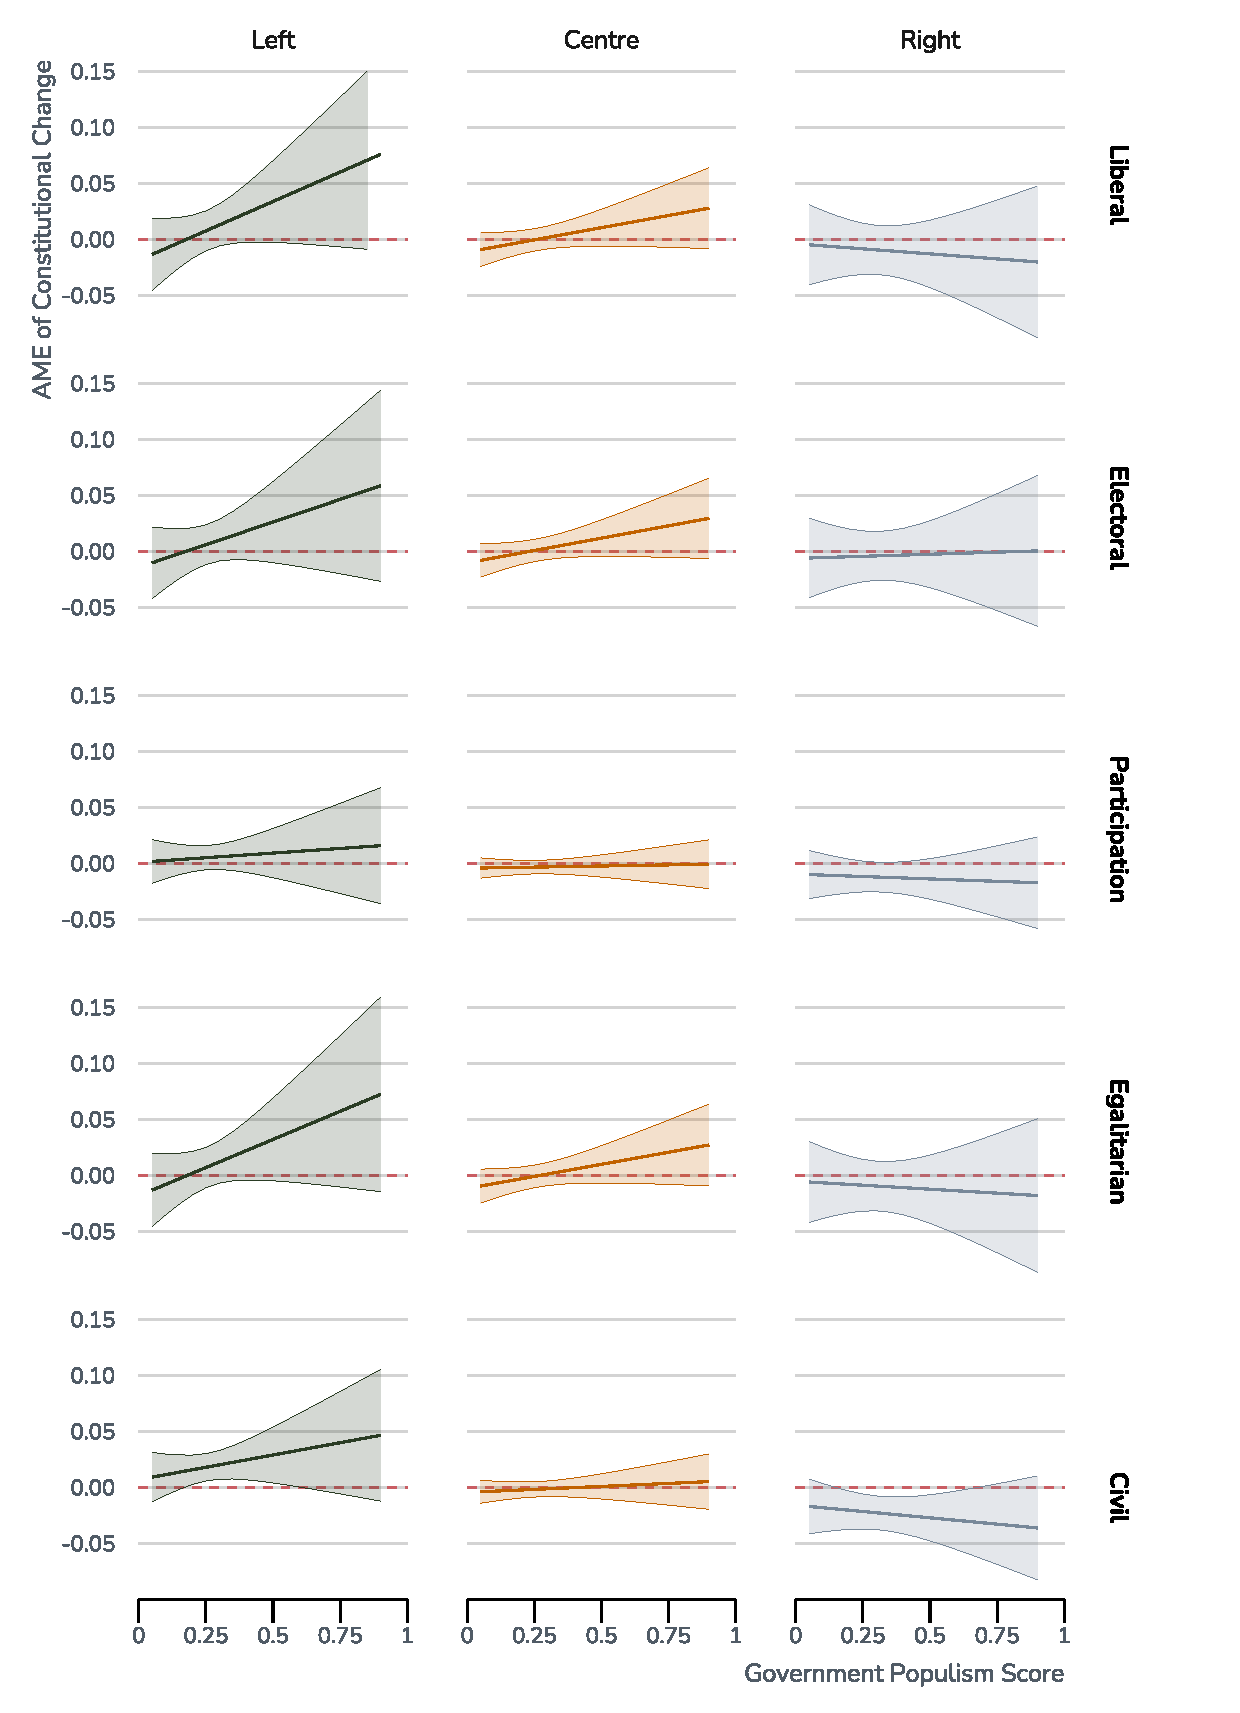
\includegraphics{results/graphs/constchange_eu.pdf}

}

\caption{\label{fig-eu}Average marginal effect of constitutional change
condititoned by government weighted populism score and ideology
(GAL-TAN) for Europe, based Table~\ref{tbl-libdem_sep} to
Table~\ref{tbl-cspart_sep}, model 3.}

\end{figure}

\begin{figure}[H]

{\centering 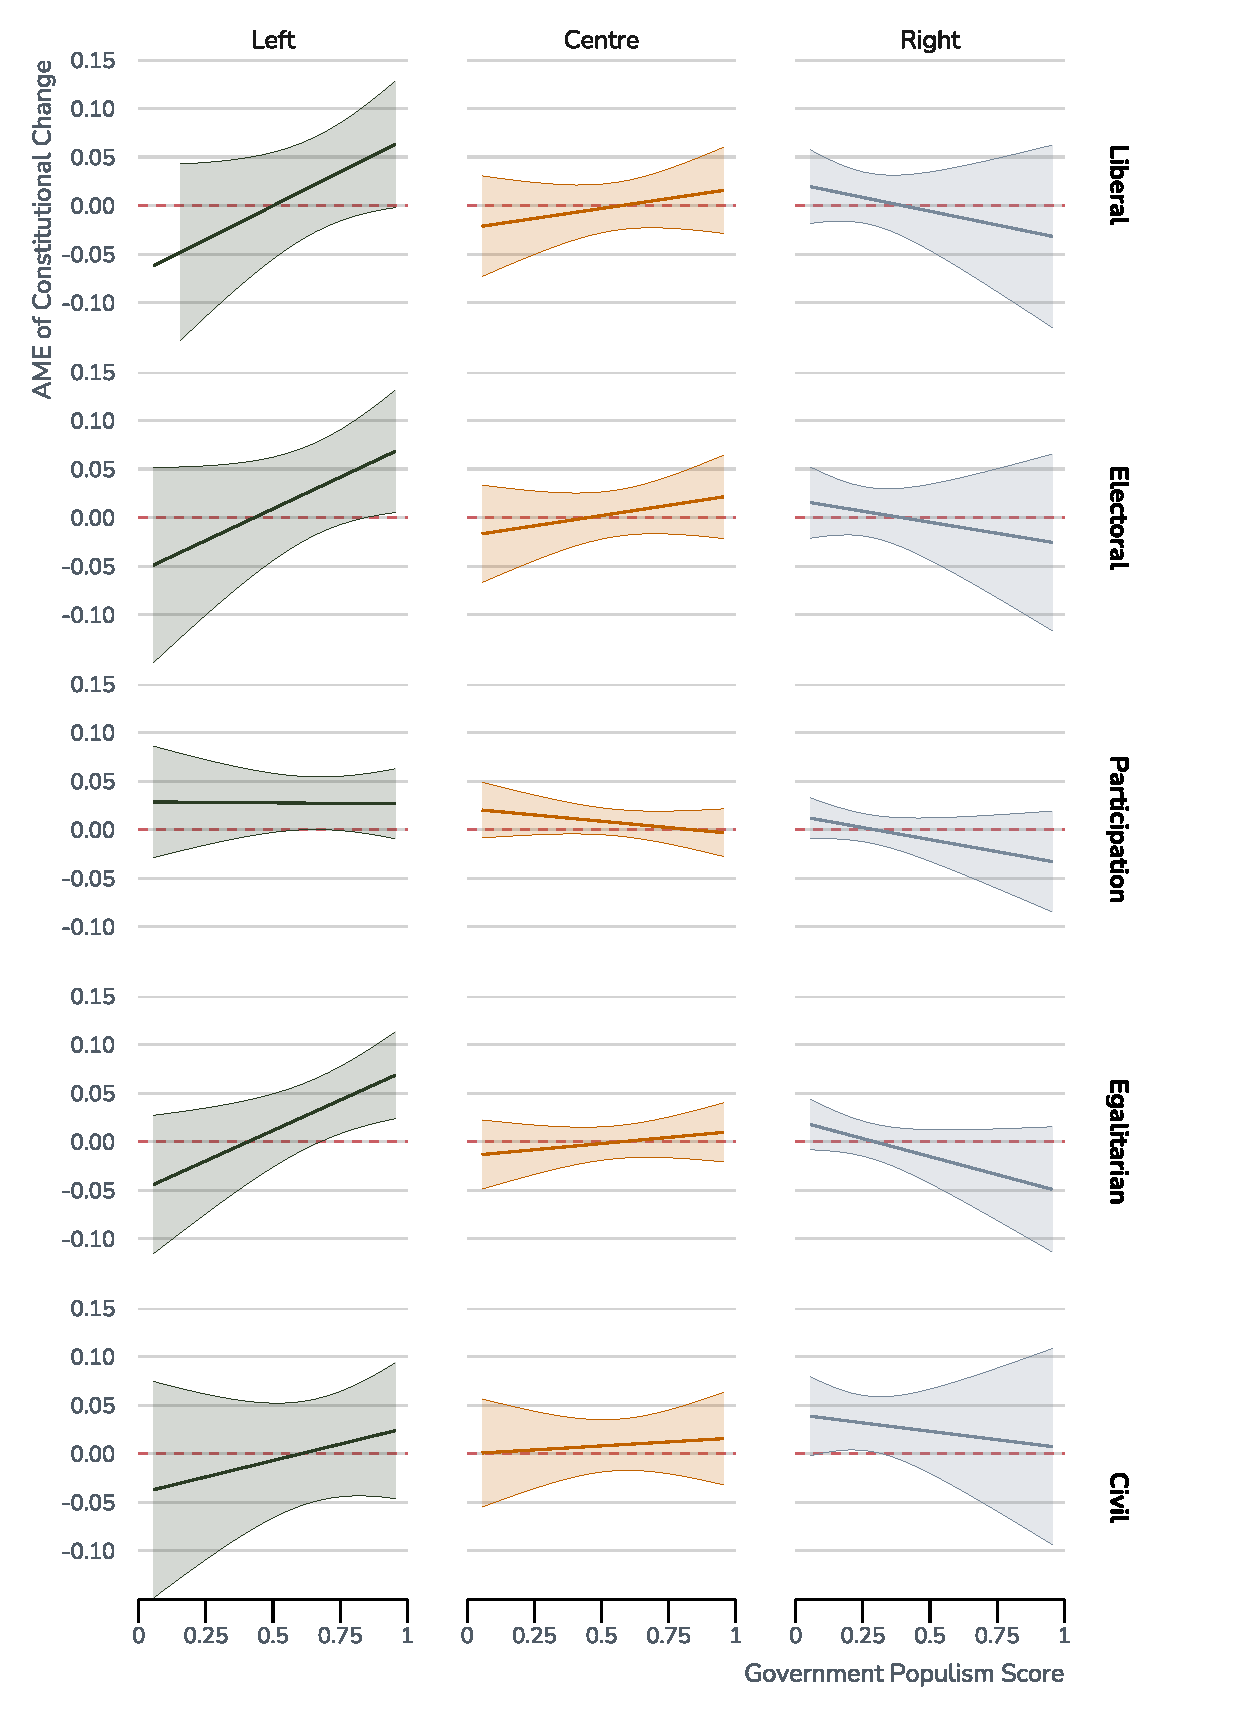
\includegraphics{results/graphs/constchange_la.pdf}

}

\caption{\label{fig-la}Average marginal effect of constitutional change
condititoned by government weighted populism score and ideology for
Latin America, based Table~\ref{tbl-libdem_sep} to
Table~\ref{tbl-cspart_sep}, model 2.}

\end{figure}

\blandscape
\renewcommand{\arraystretch}{0.5}

\hypertarget{tbl-dynamic}{}
\begin{table}
\caption{\label{tbl-dynamic}Dynamic regression models }\tabularnewline

\centering\centering\centering
\begin{tabular}[t]{lccccc}
\toprule
  & Liberal & Electoral & Participation & Egalitarian & Civil Society\\
\midrule
Populism & -0.103*** & -0.165*** & -0.139*** & -0.040** & -0.120**\\
 & {}[-0.139, -0.068] & {}[-0.215, -0.115] & {}[-0.197, -0.080] & {}[-0.068, -0.012] & {}[-0.197, -0.044]\\
Const. Change & 0.015 & 0.022 & 0.024 & 0.006 & 0.112***\\
 & {}[-0.011, 0.041] & {}[-0.015, 0.058] & {}[-0.019, 0.067] & {}[-0.013, 0.026] & {}[0.060, 0.165]\\
Dem.Scorelagged & 0.602*** & 0.582*** & 0.526*** & 0.674*** & 0.562***\\
 & {}[0.560, 0.645] & {}[0.537, 0.626] & {}[0.475, 0.578] & {}[0.634, 0.714] & {}[0.502, 0.623]\\
surplus\_size & -0.001*** & -0.001*** & 0.000*** & 0.000** & -0.001**\\
 & {}[-0.001, 0.000] & {}[-0.001, 0.000] & {}[-0.001, 0.000] & {}[-0.001, 0.000] & {}[-0.001, 0.000]\\
coalition & 0.016*** & 0.015*** & 0.004 & 0.010*** & 0.008+\\
 & {}[0.009, 0.023] & {}[0.008, 0.022] & {}[-0.001, 0.009] & {}[0.004, 0.015] & {}[0.000, 0.016]\\
Populism:Const. Change & 0.023 & 0.051 & 0.028 & 0.018 & -0.144*\\
 & {}[-0.037, 0.084] & {}[-0.043, 0.146] & {}[-0.086, 0.141] & {}[-0.031, 0.066] & {}[-0.280, -0.008]\\
Populism:Dem.Scorelagged & 0.074* & 0.168*** & 0.209*** & 0.008 & 0.106*\\
 & {}[0.013, 0.136] & {}[0.097, 0.238] & {}[0.115, 0.303] & {}[-0.042, 0.058] & {}[0.005, 0.206]\\
Const. Change:Dem.Scorelagged & -0.024 & -0.028 & -0.029 & -0.014 & -0.124***\\
 & {}[-0.063, 0.015] & {}[-0.076, 0.020] & {}[-0.098, 0.040] & {}[-0.044, 0.017] & {}[-0.189, -0.060]\\
Populism:Const. Change:Dem.Scorelagged & -0.020 & -0.053 & -0.040 & -0.002 & 0.171+\\
 & {}[-0.121, 0.082] & {}[-0.183, 0.077] & {}[-0.219, 0.138] & {}[-0.085, 0.082] & {}[-0.003, 0.345]\\
\midrule
Country FE & Yes & Yes & Yes & Yes & Yes\\
Num.Obs. & 1470 & 1470 & 1470 & 1470 & 1470\\
R2 & 0.604 & 0.597 & 0.492 & 0.560 & 0.467\\
R2 Adj. & 0.586 & 0.578 & 0.468 & 0.539 & 0.442\\
AIC & -5274.8 & -5393.3 & -6469.5 & -6046.9 & -4839.4\\
BIC & -5221.8 & -5340.4 & -6416.5 & -5993.9 & -4786.5\\
RMSE & 0.04 & 0.04 & 0.03 & 0.03 & 0.05\\
\bottomrule
\multicolumn{6}{l}{\rule{0pt}{1em}+p $<$ 0.1; *p $<$ 0.05; **p > 0.01; ***p $<$ 0.001}\\
\end{tabular}
\end{table}

\elandscape

\begin{figure}[H]

{\centering 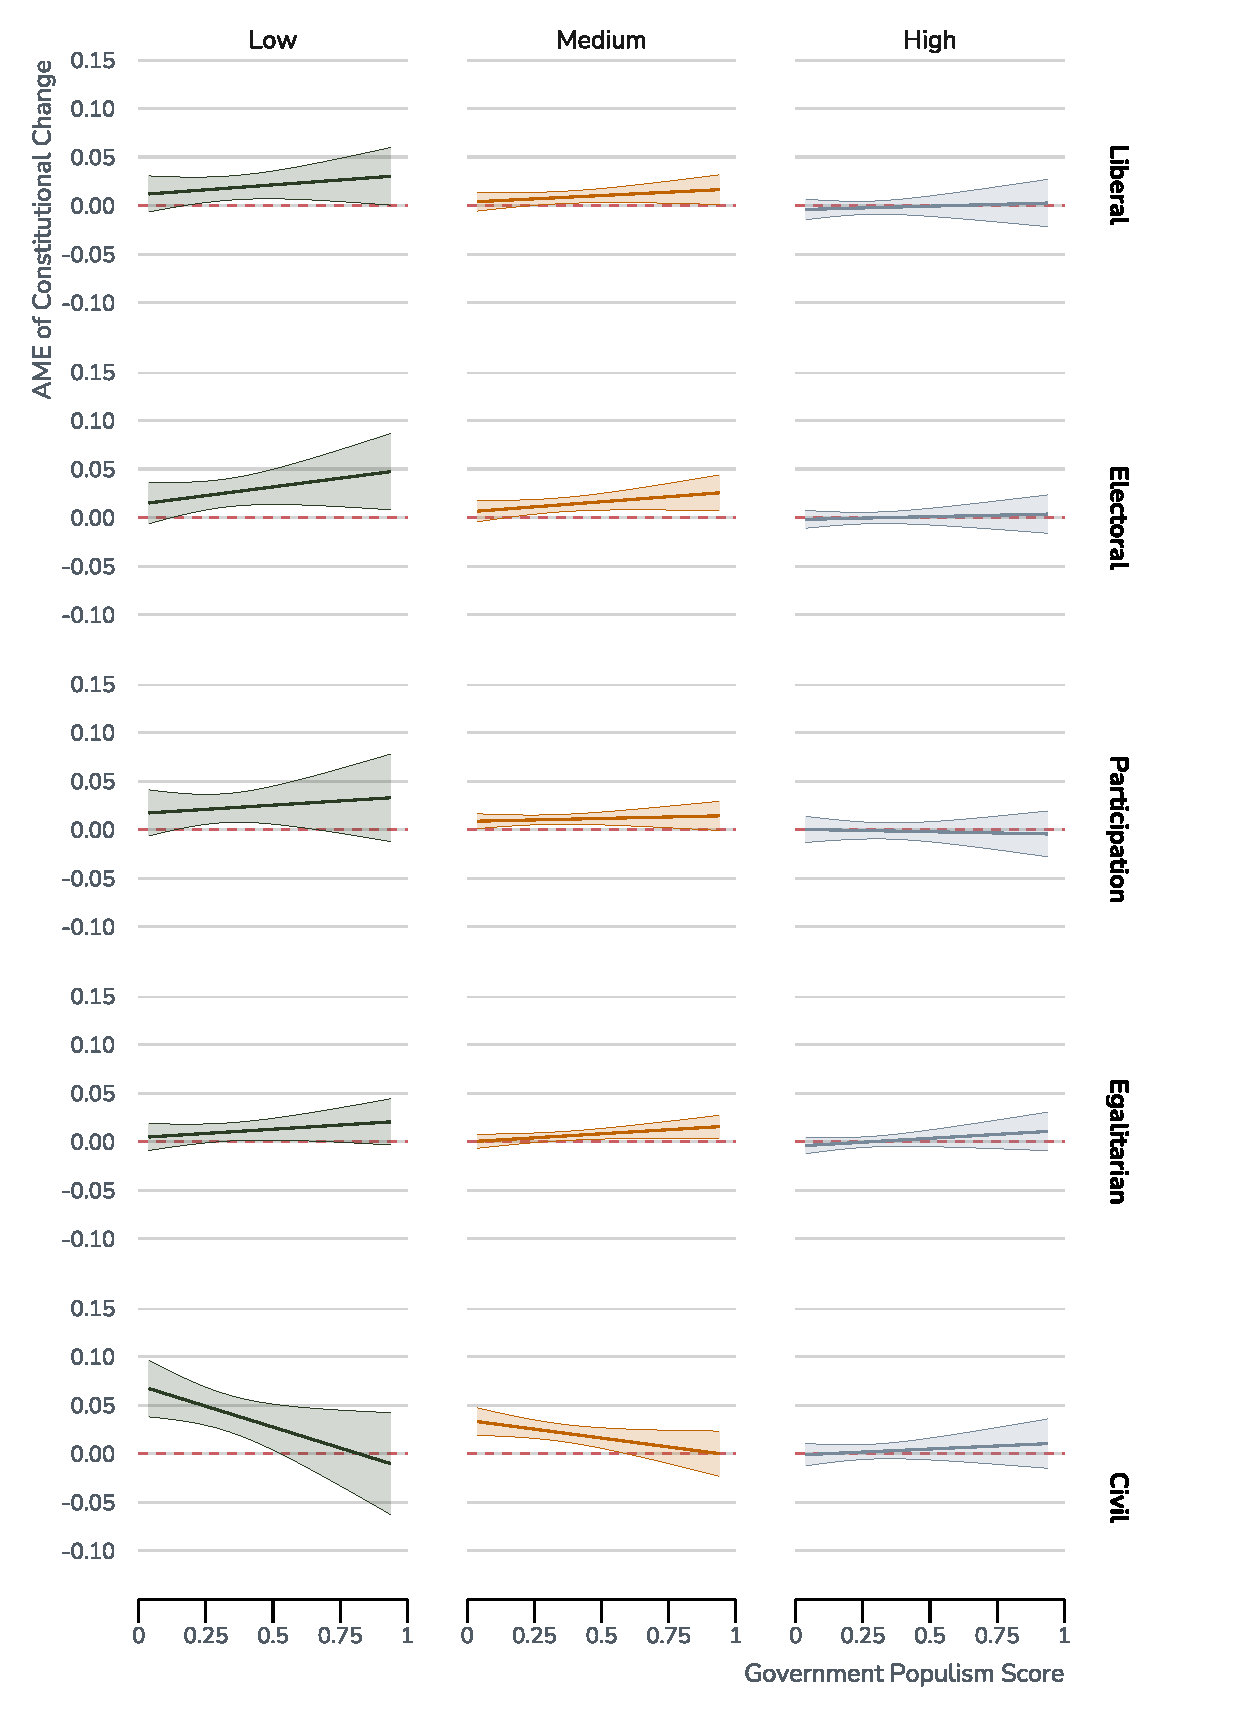
\includegraphics{results/graphs/constchange_dynamic.pdf}

}

\caption{\label{fig-dynamic}Average marginal effect of constitutional
change condititoned by government weighted populism score and lag of
democratic quality ahead, based Table~\ref{tbl-dynamic}.}

\end{figure}

\blandscape

\hypertarget{tbl-ruth}{}
\begin{table}
\caption{\label{tbl-ruth}Regression models with Ruth-Lovell \& Grahn populism coding }\tabularnewline

\centering\centering\centering
\begin{tabular}[t]{lccccc}
\toprule
  & Liberal & Electoral & Participation & Egalitarian & Civil Society\\
\midrule
Left-wing Populist & -0.122*** & -0.109*** & 0.043*** & -0.054*** & -0.037***\\
 & {}[-0.144, -0.100] & {}[-0.128, -0.089] & {}[0.029, 0.056] & {}[-0.069, -0.038] & {}[-0.057, -0.016]\\
Right-wing Populist & -0.075*** & -0.058*** & -0.007 & -0.050*** & -0.040***\\
 & {}[-0.093, -0.056] & {}[-0.075, -0.041] & {}[-0.018, 0.005] & {}[-0.064, -0.037] & {}[-0.058, -0.022]\\
Constitutional Change & 0.006 & 0.006 & 0.003 & 0.004 & 0.009*\\
 & {}[-0.002, 0.015] & {}[-0.002, 0.013] & {}[-0.002, 0.009] & {}[-0.003, 0.010] & {}[0.001, 0.017]\\
surplus\_size & -0.002*** & -0.001*** & -0.001*** & -0.001*** & -0.001***\\
 & {}[-0.002, -0.001] & {}[-0.002, -0.001] & {}[-0.001, 0.000] & {}[-0.001, 0.000] & {}[-0.002, -0.001]\\
coalition & 0.029*** & 0.024*** & 0.007* & 0.012** & 0.012*\\
 & {}[0.018, 0.040] & {}[0.014, 0.034] & {}[0.000, 0.014] & {}[0.004, 0.020] & {}[0.002, 0.023]\\
Left-wing Populist:Constitutional Change & 0.022 & 0.036* & 0.009 & 0.035* & 0.016\\
 & {}[-0.016, 0.059] & {}[0.002, 0.069] & {}[-0.015, 0.033] & {}[0.008, 0.062] & {}[-0.020, 0.051]\\
Right-wing Populist:Constitutional Change & -0.017 & -0.013 & -0.007 & -0.021+ & -0.025\\
 & {}[-0.049, 0.015] & {}[-0.042, 0.015] & {}[-0.027, 0.013] & {}[-0.044, 0.002] & {}[-0.056, 0.005]\\
\midrule
Country FE & Yes & Yes & Yes & Yes & Yes\\
Num.Obs. & 1139 & 1139 & 1139 & 1139 & 1139\\
R2 & 0.217 & 0.192 & 0.057 & 0.134 & 0.072\\
R2 Adj. & 0.179 & 0.154 & 0.012 & 0.092 & 0.028\\
AIC & -3383.3 & -3620.5 & -4420.8 & -4118.9 & -3484.0\\
BIC & -3343.0 & -3580.2 & -4380.5 & -4078.6 & -3443.7\\
RMSE & 0.05 & 0.05 & 0.03 & 0.04 & 0.05\\
\bottomrule
\multicolumn{6}{l}{\rule{0pt}{1em}+p $<$ 0.1; *p $<$ 0.05; **p > 0.01; ***p $<$ 0.001}\\
\end{tabular}
\end{table}

\renewcommand{\arraystretch}{0.5}

\hypertarget{tbl-leadlibdem}{}
\begin{table}
\caption{\label{tbl-leadlibdem}Regression models on liberal democracy for different leads }\tabularnewline

\centering\centering\centering
\begin{tabular}[t]{lcccc}
\toprule
  & (1) & (2) & (3) & (4)\\
\midrule
Populism & -0.101*** & -0.079*** & -0.061** & -0.038+\\
 & {}[-0.139, -0.063] & {}[-0.117, -0.042] & {}[-0.099, -0.024] & {}[-0.077, 0.000]\\
Const. Change & 0.000 & 0.005 & 0.010 & 0.018*\\
 & {}[-0.017, 0.016] & {}[-0.011, 0.022] & {}[-0.006, 0.027] & {}[0.001, 0.034]\\
Left-Right & 0.036*** & 0.040*** & 0.041*** & 0.037***\\
 & {}[0.018, 0.054] & {}[0.022, 0.057] & {}[0.023, 0.059] & {}[0.020, 0.055]\\
Surplus & -0.002*** & -0.002*** & -0.002*** & -0.001***\\
 & {}[-0.003, -0.002] & {}[-0.003, -0.002] & {}[-0.002, -0.001] & {}[-0.002, -0.001]\\
Coalition & 0.047*** & 0.038*** & 0.030*** & 0.024***\\
 & {}[0.037, 0.058] & {}[0.027, 0.048] & {}[0.019, 0.040] & {}[0.013, 0.034]\\
Populism:Const. Change & 0.015 & -0.020 & -0.041 & -0.096***\\
 & {}[-0.036, 0.067] & {}[-0.071, 0.032] & {}[-0.092, 0.011] & {}[-0.148, -0.044]\\
Populism:Left-Right & -0.041+ & -0.070** & -0.086*** & -0.096***\\
 & {}[-0.089, 0.006] & {}[-0.117, -0.024] & {}[-0.132, -0.040] & {}[-0.144, -0.049]\\
Const. Change:Left-Right & -0.026+ & -0.031* & -0.039** & -0.047***\\
 & {}[-0.053, 0.001] & {}[-0.057, -0.004] & {}[-0.066, -0.013] & {}[-0.074, -0.021]\\
Populism:Const. Change:Left-Right & 0.063+ & 0.100** & 0.125*** & 0.167***\\
 & {}[-0.007, 0.133] & {}[0.031, 0.170] & {}[0.055, 0.194] & {}[0.098, 0.237]\\
\midrule
Country FE & Yes & Yes & Yes & Yes\\
Num.Obs. & 1539 & 1482 & 1425 & 1369\\
R2 & 0.186 & 0.170 & 0.147 & 0.127\\
R2 Adj. & 0.150 & 0.132 & 0.106 & 0.083\\
AIC & -4176.2 & -4143.5 & -4072.2 & -3960.6\\
BIC & -4122.8 & -4090.5 & -4019.6 & -3908.4\\
RMSE & 0.06 & 0.06 & 0.06 & 0.06\\
\bottomrule
\multicolumn{5}{l}{\rule{0pt}{1em}+p $<$ 0.1; *p $<$ 0.05; **p > 0.01; ***p $<$ 0.001}\\
\end{tabular}
\end{table}

\hypertarget{tbl-leadpartip}{}
\begin{table}
\caption{\label{tbl-leadpartip}Regression models on participation for different leads }\tabularnewline

\centering\centering\centering
\begin{tabular}[t]{lcccc}
\toprule
  & (1) & (2) & (3) & (4)\\
\midrule
Populism & -0.004 & -0.001 & -0.001 & 0.002\\
 & {}[-0.027, 0.019] & {}[-0.024, 0.022] & {}[-0.024, 0.022] & {}[-0.022, 0.025]\\
Const. Change & 0.004 & 0.007 & 0.008 & 0.010+\\
 & {}[-0.006, 0.014] & {}[-0.003, 0.017] & {}[-0.002, 0.018] & {}[-0.001, 0.020]\\
Left-Right & -0.001 & 0.005 & 0.007 & 0.006\\
 & {}[-0.012, 0.011] & {}[-0.006, 0.016] & {}[-0.004, 0.018] & {}[-0.005, 0.017]\\
Surplus & -0.001*** & -0.001*** & -0.001*** & -0.001***\\
 & {}[-0.001, -0.001] & {}[-0.001, -0.001] & {}[-0.001, -0.001] & {}[-0.001, 0.000]\\
Coalition & 0.013*** & 0.012*** & 0.012*** & 0.011**\\
 & {}[0.007, 0.020] & {}[0.005, 0.018] & {}[0.005, 0.018] & {}[0.004, 0.017]\\
Populism:Const. Change & -0.001 & -0.022 & -0.030+ & -0.039*\\
 & {}[-0.033, 0.030] & {}[-0.054, 0.009] & {}[-0.062, 0.002] & {}[-0.071, -0.007]\\
Populism:Left-Right & 0.019 & 0.004 & -0.001 & -0.004\\
 & {}[-0.010, 0.048] & {}[-0.024, 0.033] & {}[-0.030, 0.027] & {}[-0.033, 0.025]\\
Const. Change:Left-Right & -0.003 & -0.009 & -0.012 & -0.015+\\
 & {}[-0.019, 0.013] & {}[-0.025, 0.007] & {}[-0.028, 0.004] & {}[-0.031, 0.001]\\
Populism:Const. Change:Left-Right & 0.004 & 0.030 & 0.043* & 0.057**\\
 & {}[-0.038, 0.047] & {}[-0.013, 0.072] & {}[0.000, 0.086] & {}[0.014, 0.100]\\
\midrule
Country FE & Yes & Yes & Yes & Yes\\
Num.Obs. & 1539 & 1482 & 1425 & 1369\\
R2 & 0.051 & 0.048 & 0.044 & 0.039\\
R2 Adj. & 0.009 & 0.004 & -0.002 & -0.009\\
AIC & -5696.7 & -5596.2 & -5454.6 & -5299.9\\
BIC & -5643.3 & -5543.2 & -5401.9 & -5247.7\\
RMSE & 0.04 & 0.04 & 0.04 & 0.03\\
\bottomrule
\multicolumn{5}{l}{\rule{0pt}{1em}+p $<$ 0.1; *p $<$ 0.05; **p > 0.01; ***p $<$ 0.001}\\
\end{tabular}
\end{table}

\hypertarget{tbl-leadpolyarchy}{}
\begin{table}
\caption{\label{tbl-leadpolyarchy}Regression models on polyarchy for different leads }\tabularnewline

\centering\centering\centering
\begin{tabular}[t]{lcccc}
\toprule
  & (1) & (2) & (3) & (4)\\
\midrule
Populism & -0.076*** & -0.057** & -0.047* & -0.026\\
 & {}[-0.112, -0.039] & {}[-0.093, -0.022] & {}[-0.082, -0.011] & {}[-0.063, 0.011]\\
Const. Change & -0.001 & 0.006 & 0.012 & 0.020*\\
 & {}[-0.017, 0.015] & {}[-0.009, 0.022] & {}[-0.004, 0.027] & {}[0.005, 0.036]\\
Left-Right & 0.034*** & 0.038*** & 0.040*** & 0.038***\\
 & {}[0.017, 0.052] & {}[0.021, 0.055] & {}[0.024, 0.057] & {}[0.021, 0.055]\\
Surplus & -0.002*** & -0.002*** & -0.002*** & -0.002***\\
 & {}[-0.003, -0.002] & {}[-0.002, -0.002] & {}[-0.002, -0.001] & {}[-0.002, -0.001]\\
Coalition & 0.044*** & 0.035*** & 0.029*** & 0.023***\\
 & {}[0.033, 0.054] & {}[0.025, 0.045] & {}[0.019, 0.039] & {}[0.013, 0.034]\\
Populism:Const. Change & 0.021 & -0.015 & -0.030 & -0.093***\\
 & {}[-0.029, 0.070] & {}[-0.064, 0.034] & {}[-0.080, 0.019] & {}[-0.143, -0.043]\\
Populism:Left-Right & -0.047* & -0.073** & -0.089*** & -0.102***\\
 & {}[-0.092, -0.001] & {}[-0.118, -0.029] & {}[-0.133, -0.045] & {}[-0.147, -0.057]\\
Const. Change:Left-Right & -0.021 & -0.026* & -0.036** & -0.046***\\
 & {}[-0.047, 0.005] & {}[-0.051, -0.001] & {}[-0.061, -0.012] & {}[-0.071, -0.021]\\
Populism:Const. Change:Left-Right & 0.051 & 0.077* & 0.104** & 0.152***\\
 & {}[-0.016, 0.118] & {}[0.011, 0.144] & {}[0.037, 0.170] & {}[0.086, 0.219]\\
\midrule
Country FE & Yes & Yes & Yes & Yes\\
Num.Obs. & 1539 & 1482 & 1425 & 1369\\
R2 & 0.165 & 0.155 & 0.142 & 0.131\\
R2 Adj. & 0.128 & 0.116 & 0.101 & 0.087\\
AIC & -4309.6 & -4284.4 & -4210.0 & -4080.8\\
BIC & -4256.2 & -4231.4 & -4157.4 & -4028.6\\
RMSE & 0.06 & 0.06 & 0.05 & 0.05\\
\bottomrule
\multicolumn{5}{l}{\rule{0pt}{1em}+p $<$ 0.1; *p $<$ 0.05; **p > 0.01; ***p $<$ 0.001}\\
\end{tabular}
\end{table}

\hypertarget{tbl-leadcspart}{}
\begin{table}
\caption{\label{tbl-leadcspart}Regression models on civil society for different leads }\tabularnewline

\centering\centering\centering
\begin{tabular}[t]{lcccc}
\toprule
  & (1) & (2) & (3) & (4)\\
\midrule
Populism & -0.054** & -0.045* & -0.031 & 0.000\\
 & {}[-0.092, -0.015] & {}[-0.084, -0.007] & {}[-0.069, 0.007] & {}[-0.038, 0.039]\\
Const. Change & 0.012 & 0.017* & 0.018* & 0.029***\\
 & {}[-0.005, 0.029] & {}[0.000, 0.034] & {}[0.002, 0.035] & {}[0.013, 0.046]\\
Left-Right & 0.023* & 0.021* & 0.024** & 0.022*\\
 & {}[0.004, 0.041] & {}[0.002, 0.039] & {}[0.006, 0.042] & {}[0.004, 0.040]\\
Surplus & -0.002*** & -0.002*** & -0.002*** & -0.001***\\
 & {}[-0.003, -0.002] & {}[-0.003, -0.002] & {}[-0.002, -0.001] & {}[-0.002, -0.001]\\
Coalition & 0.031*** & 0.027*** & 0.022*** & 0.018***\\
 & {}[0.020, 0.042] & {}[0.016, 0.038] & {}[0.011, 0.033] & {}[0.008, 0.029]\\
Populism:Const. Change & -0.005 & -0.047+ & -0.055* & -0.111***\\
 & {}[-0.058, 0.048] & {}[-0.100, 0.007] & {}[-0.108, -0.002] & {}[-0.163, -0.059]\\
Populism:Left-Right & -0.027 & -0.037 & -0.056* & -0.073**\\
 & {}[-0.076, 0.021] & {}[-0.085, 0.011] & {}[-0.103, -0.009] & {}[-0.120, -0.026]\\
Const. Change:Left-Right & -0.010 & -0.014 & -0.028* & -0.037**\\
 & {}[-0.037, 0.018] & {}[-0.041, 0.013] & {}[-0.054, -0.001] & {}[-0.063, -0.010]\\
Populism:Const. Change:Left-Right & 0.021 & 0.053 & 0.096** & 0.146***\\
 & {}[-0.050, 0.093] & {}[-0.019, 0.125] & {}[0.025, 0.167] & {}[0.077, 0.216]\\
\midrule
Country FE & Yes & Yes & Yes & Yes\\
Num.Obs. & 1539 & 1482 & 1425 & 1369\\
R2 & 0.112 & 0.104 & 0.090 & 0.077\\
R2 Adj. & 0.073 & 0.063 & 0.046 & 0.031\\
AIC & -4106.8 & -4046.2 & -4004.7 & -3960.1\\
BIC & -4053.5 & -3993.2 & -3952.1 & -3907.9\\
RMSE & 0.06 & 0.06 & 0.06 & 0.06\\
\bottomrule
\multicolumn{5}{l}{\rule{0pt}{1em}+p $<$ 0.1; *p $<$ 0.05; **p > 0.01; ***p $<$ 0.001}\\
\end{tabular}
\end{table}

\hypertarget{tbl-leadegaldem}{}
\begin{table}
\caption{\label{tbl-leadegaldem}Regression models on egalitarian democracy for different leads }\tabularnewline

\centering\centering\centering
\begin{tabular}[t]{lcccc}
\toprule
  & (1) & (2) & (3) & (4)\\
\midrule
Populism & -0.066*** & -0.054*** & -0.047*** & -0.032*\\
 & {}[-0.094, -0.038] & {}[-0.082, -0.027] & {}[-0.075, -0.019] & {}[-0.061, -0.004]\\
Const. Change & 0.002 & 0.006 & 0.009 & 0.016**\\
 & {}[-0.011, 0.014] & {}[-0.006, 0.019] & {}[-0.003, 0.022] & {}[0.004, 0.029]\\
Left-Right & 0.022** & 0.023*** & 0.023*** & 0.020**\\
 & {}[0.008, 0.035] & {}[0.010, 0.036] & {}[0.010, 0.036] & {}[0.007, 0.034]\\
Surplus & -0.001*** & -0.001*** & -0.001*** & -0.001***\\
 & {}[-0.002, -0.001] & {}[-0.002, -0.001] & {}[-0.002, -0.001] & {}[-0.001, -0.001]\\
Coalition & 0.030*** & 0.025*** & 0.021*** & 0.017***\\
 & {}[0.022, 0.038] & {}[0.017, 0.033] & {}[0.013, 0.029] & {}[0.010, 0.025]\\
Populism:Const. Change & -0.004 & -0.027 & -0.037+ & -0.080***\\
 & {}[-0.042, 0.034] & {}[-0.065, 0.011] & {}[-0.076, 0.002] & {}[-0.119, -0.041]\\
Populism:Left-Right & -0.011 & -0.027 & -0.035* & -0.043*\\
 & {}[-0.047, 0.024] & {}[-0.062, 0.007] & {}[-0.069, 0.000] & {}[-0.078, -0.008]\\
Const. Change:Left-Right & -0.020* & -0.020* & -0.026* & -0.035***\\
 & {}[-0.040, 0.000] & {}[-0.040, -0.001] & {}[-0.045, -0.006] & {}[-0.055, -0.016]\\
Populism:Const. Change:Left-Right & 0.070** & 0.084** & 0.094*** & 0.131***\\
 & {}[0.017, 0.122] & {}[0.032, 0.135] & {}[0.042, 0.146] & {}[0.080, 0.183]\\
\midrule
Country FE & Yes & Yes & Yes & Yes\\
Num.Obs. & 1539 & 1482 & 1425 & 1369\\
R2 & 0.137 & 0.128 & 0.114 & 0.107\\
R2 Adj. & 0.099 & 0.088 & 0.071 & 0.062\\
AIC & -5095.5 & -5026.5 & -4904.9 & -4763.5\\
BIC & -5042.1 & -4973.4 & -4852.3 & -4711.2\\
RMSE & 0.05 & 0.04 & 0.04 & 0.04\\
\bottomrule
\multicolumn{5}{l}{\rule{0pt}{1em}+p $<$ 0.1; *p $<$ 0.05; **p > 0.01; ***p $<$ 0.001}\\
\end{tabular}
\end{table}

\elandscape

\blandscape

\begin{figure}[H]

{\centering 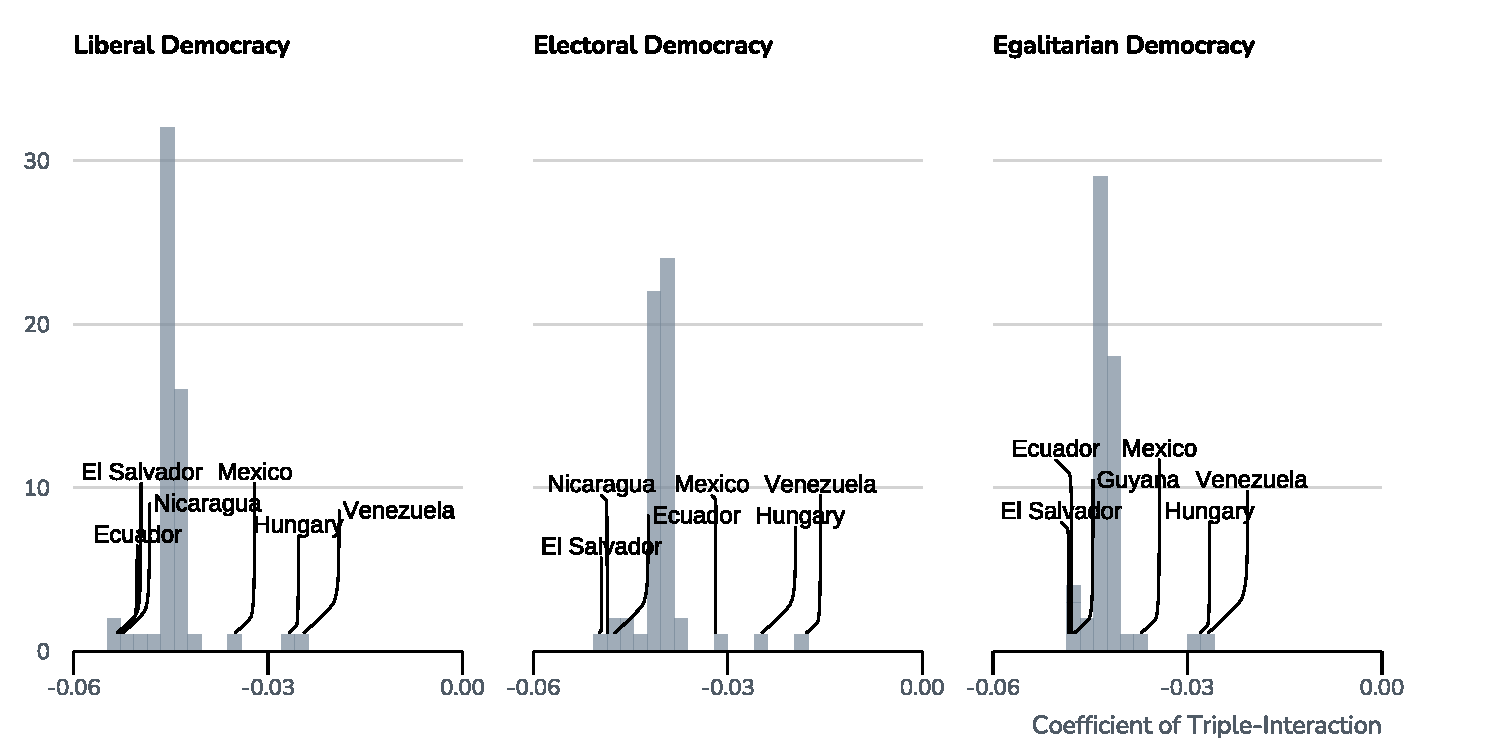
\includegraphics{results/graphs/jackknife_plots.pdf}

}

\caption{\label{fig-jackknife1}Coefficients of triple-Interaction effect
in jackknife-model.}

\end{figure}

\begin{figure}[H]

{\centering 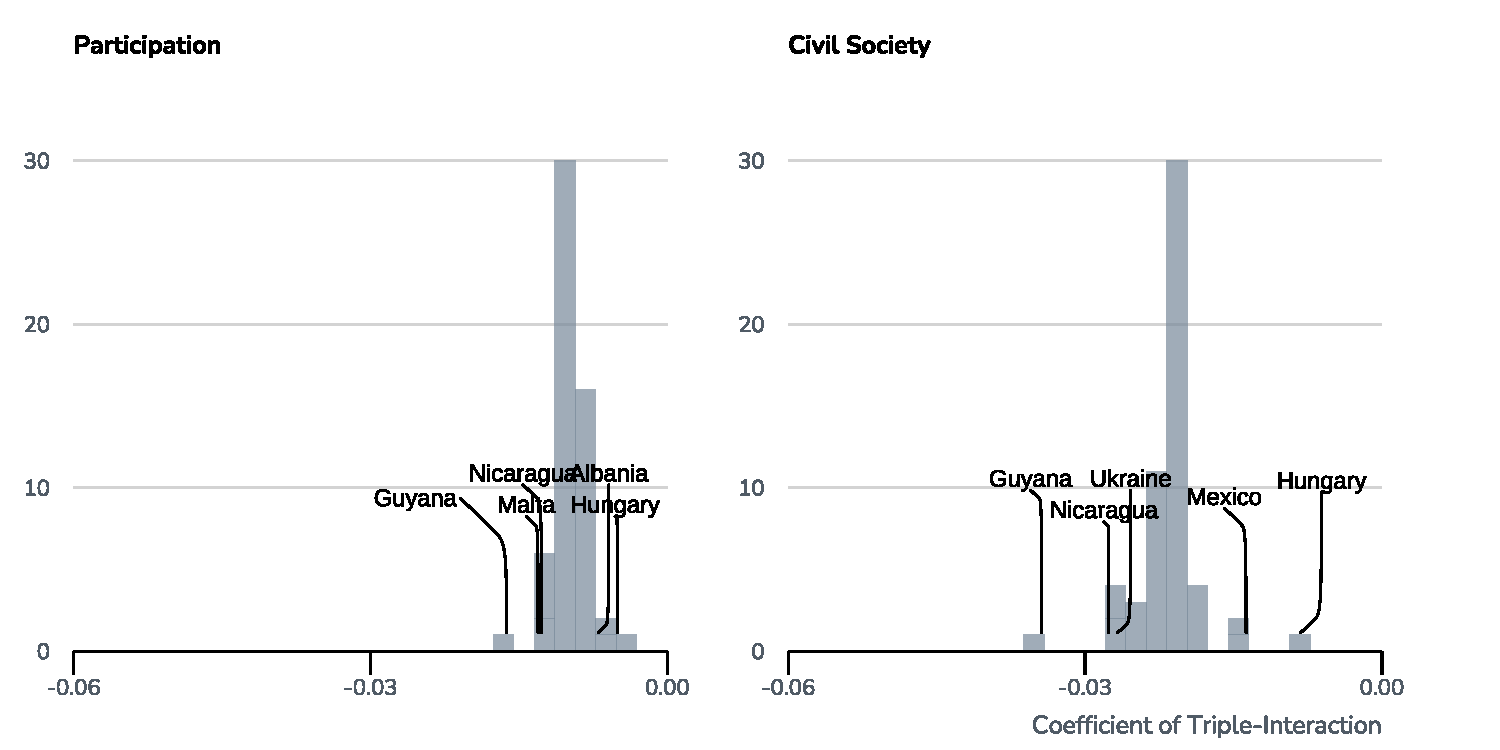
\includegraphics{results/graphs/jackknife_plots2.pdf}

}

\caption{\label{fig-jackknife2}Coefficients of triple-interaction effect
in jackknife-model.}

\end{figure}

\elandscape



\end{document}
